\documentclass[a4paper,12pt]{article}

\input{tools/packages.tex}

\colorlet{punct}{red!60!black}
\definecolor{background}{HTML}{EEEEEE}
\definecolor{delim}{RGB}{20,105,176}
\colorlet{numb}{magenta!60!black}

\def\mylstdelim#1#2#3{
    \def\endlstdelim{\textcolor{#3}{#2}\egroup}
    \textcolor{#3}{#1}\bgroup\aftergroup\endlstdelim
}

\lstdefinelanguage{json}{
    basicstyle=\normalfont\ttfamily,
    numbers=left,
    numberstyle=\scriptsize,
    stepnumber=1,
    numbersep=8pt,
    showstringspaces=false,
    breaklines=true,
    frame=lines,
    backgroundcolor=\color{background},
    moredelim = **[is][{\mylstdelim{[}{]}{delim}}]{[}{]},
    moredelim = **[is][{\mylstdelim{\{}{\}}{delim}}]{\{}{\}},
    literate=
     *{0}{{{\color{numb}0}}}{1}
      {1}{{{\color{numb}1}}}{1}
      {2}{{{\color{numb}2}}}{1}
      {3}{{{\color{numb}3}}}{1}
      {4}{{{\color{numb}4}}}{1}
      {5}{{{\color{numb}5}}}{1}
      {6}{{{\color{numb}6}}}{1}
      {7}{{{\color{numb}7}}}{1}
      {8}{{{\color{numb}8}}}{1}
      {9}{{{\color{numb}9}}}{1}
      {:}{{{\color{punct}{:}}}}{1}
      {,}{{{\color{punct}{,}}}}{1}
}

\lstnewenvironment{bashcode}[1][]{
    \lstset{
        basicstyle=\ttfamily,
        columns=fullflexible,
        language=bash,
        keepspaces=true,
        breaklines=true,
        breakatwhitespace=true,
        prebreak=\char`\\, % Example character to indicate a break
        showstringspaces=false,
        belowskip=-1em,
        #1 % Any additional settings you want to pass
    }
}{}

%RBG FFD33E / C95D40
\definecolor{upcorange}{HTML}{FFD33E}
\hypersetup{allcolors=black}

% probably a good idea for the nomenclature entries:
\acsetup{
  first-style=long-short, %footnote,
  subsequent-style=short,
  pages/display=all,
  list/heading=none
}

%%%% PAGE STYLE %%%%%
\usepackage{fancyhdr}
\pagestyle{fancy}
\setlength{\footskip}{68pt}
\fancyhf{}
\lhead{\includegraphics[height=1.2cm]{figures/logos/upclogo.png}}
\rhead{\includegraphics[height=1.2cm]{figures/logos/logo_telecos.png}}
\rfoot{\thepage{}}

\renewcommand{\footrulewidth}{0.4pt}
%\futurelet\TMPfootrule\def\footrule{{\color{upcorange}\TMPfootrule}}
\futurelet\TMPfootrule\def\footrule{{\color{gray!80}\TMPfootrule}}
\renewcommand{\headrulewidth}{0.4pt}
\renewcommand{\headrule}{\hbox to \headwidth{%
%\color{upcorange}\leaders\hrule height \headrulewidth\hfill}}
\color{gray!80}\leaders\hrule height \headrulewidth\hfill}}
%\renewcommand*\ShowFrameColor{\color{red}}

\usepackage{footmisc}


% class `abbrev': abbreviations:

\DeclareAcronym{AP}{
  short = AP ,
  long  = Average Precision
}

\DeclareAcronym{AssA}{
  short = AssA ,
  long  = Association Accuracy
}

\DeclareAcronym{BoT}{
  short = BoT ,
  long  = Bag of Tricks
}

\DeclareAcronym{BYTE}{
  short = BYTE ,
  long  = ByteTrack
}

\DeclareAcronym{CIoU}{
  short = CIoU ,
  long  = Complete Intersection over Union
}

\DeclareAcronym{CNN}{
  short = CNN ,
  long  = Convolutional Neural Network
}

\DeclareAcronym{CEAB}{
  short = CEAB ,
  long = Centro de Estudios Avanzados de Blanes
}

\DeclareAcronym{CSIC}{
  short = CSIC ,
  long  = Consejo Superior de Investigaciones Científicas
}

\DeclareAcronym{CSV}{
  short = CSV ,
  long  = Comma-Separated Values
}

\DeclareAcronym{CVAT}{
  short = CVAT ,
  long = Computer Vision Annotation Tool
}

\DeclareAcronym{DetA}{
  short = DetA ,
  long  = Detection Accuracy
}

\DeclareAcronym{ECC}{
  short = ECC ,
  long  = Enhanced Correlation Coefficient
}

\DeclareAcronym{EMA}{
  short = EMA ,
  long  = Exponential Moving Average
}

\DeclareAcronym{FN}{
  short = FN ,
  long  = False Negatives
}

\DeclareAcronym{FNA}{
  short = FNA ,
  long  = False Negatives Associations
}

\DeclareAcronym{FP}{
  short = FP ,
  long  = False Positives
}

\DeclareAcronym{FPA}{
  short = FPA ,
  long  = False Positives Associations
}

\DeclareAcronym{DIoU}{
  short = DIoU ,
  long  = Distance Intersection over Union
}

\DeclareAcronym{GIoU}{
  short = GIoU ,
  long  = Generalized Intersection over Union
}

\DeclareAcronym{GSI}{
  short = GSI ,
  long  = Gaussian-Smoothed Interpolation
}

\DeclareAcronym{HOTA}{
  short = HOTA ,
  long  = Higher Order Tracking Accuracy
}

\DeclareAcronym{IoO}{
  short = IoO ,
  long  = Inner over Outer
}

\DeclareAcronym{IoU}{
  short = IoU ,
  long  = Intersection over Union
}

\DeclareAcronym{KNN}{
  short = KNN ,
  long  = K-Nearest Neighbours
}

\DeclareAcronym{LocA}{
  short = LocA ,
  long  = Localization Accuracy
}

\DeclareAcronym{mAP}{
  short = mAP ,
  long  = Mean Average Precision
}

\DeclareAcronym{MOT}{
  short = MOT ,
  long  = Multiple Object Tracking
}

\DeclareAcronym{MSE}{
  short = MSE ,
  long  = Mean Squared Error
}

\DeclareAcronym{PCA}{
  short = PCA ,
  long  = Principal Component Analysis
}

\DeclareAcronym{OC-SORT}{
  short = OC-SORT ,
  long  = Observation-Centric SORT
}

\DeclareAcronym{SAHI}{
  short = SAHI ,
  long = Slicing Aided Hyper Inference
}

\DeclareAcronym{SORT}{
  short = SORT ,
  long  = Simple Online and Realtime Tracking
}

\DeclareAcronym{TN}{
  short = TN ,
  long  = True Negatives
}

\DeclareAcronym{TNA}{
  short = TNA ,
  long  = True Negatives Associations
}

\DeclareAcronym{TP}{
  short = TP ,
  long  = True Positives
}

\DeclareAcronym{TPA}{
  short = TPA ,
  long  = True Positives Associations
}

\DeclareAcronym{TSC}{
  short = TSC ,
  long  = Teoria del Senyal i Comunicacions
}

\DeclareAcronym{TSV}{
  short = TSV ,
  long  = Tab-Separated Values
}

\DeclareAcronym{UPC}{
  short = UPC ,
  long  = Universitat Politècnica de Catalunya
}

\DeclareAcronym{WandB}{
  short = WandB ,
  long  = Weights and Bias
}

\DeclareAcronym{YOLO}{
  short = YOLO ,
  long = You Only Look Once
}

\DeclareAcronym{YOLOv8}{
  short = YOLOv8 ,
  long = You Only Look Once version 8
}

\DeclareAcronym{YOLOv8n}{
  short = YOLOv8n ,
  long = You Only Look Once version 8 nano
}


\begin{document}

%%% COVER %%%

% telecosBCN logo on the bottom of the Cover
\fancypagestyle{alim}{
    \fancyhf{}\renewcommand{\headrulewidth}{0pt}
    \cfoot{\includegraphics[height=2.2cm]{figures/logos/logo_telecos.png}}
}
\thispagestyle{empty}

\begin{center}

    { % UPC - telecosBCN logos at the top of the Cover
    \sffamily
    \resizebox{0.8\textwidth}{!}{\includegraphics{figures/logos/upc_completo+telecos.png}}\\
    \vspace{1cm}

    { % TITLE
    \Huge 	Computer vision for ant tracking\\
    \LARGE  A tool for advancing collective behavior research
    }

    \vspace{0.5cm}
    {\color{black}\hrule height 1pt}
    \vspace{1cm}

    { % Document definition and author
    \large{
        Master Thesis\\
        submitted to the Faculty of the \\
        Escola T\`ecnica d'Enginyeria de Telecomunicaci\'o de Barcelona \\
        Universitat Polit\`ecnica de Catalunya \\
        by\\
        \vspace{0.4cm}
        % NAME
        Ignasi Nogueiras Marco
        }
    }

    \vspace{1.5cm}

    { % MASTER
    In partial fulfillment\\
    of the requirements for the master in\\
    \textit{Master's degree in Telecommunications} \textbf{ENGINEERING} \textit{(MET)}\\
    \textit{multimedia specialty}
    }

    \vspace{2cm}

    {{Advisor: Josep Ramon Morros Rubió}} \\
    {{Barcelona, Date 10-02-2023}}
    \thispagestyle{alim}
    }

\end{center}

%%% INDEX %%%
\newpage
\tableofcontents

%%% REVISION %%%
\newpage
\section*{Revision history and approval record}

\selectlanguage{english}
\foreignlanguage{english}

\begin{center}
    \tablefirsthead{}
    \tablehead{}
    \tabletail{}
    \tablelasttail{}
    % Each column has a \tabcolsep at the left and the right (2 per column)
    % so \textwidth-5cm-6\tabcolsep is table_width - other cells width - 2 * num_cells * \tabcolsep
    \begin{supertabular*}{\textwidth}{|m{2cm}|m{3cm}|m{\dimexpr \textwidth-5cm-6\tabcolsep}|} 
        \hline 

        \textbf{Revision} & \textbf{Date} & \textbf{Purpose}\\
        
        \hline
        
        0 & 13/03/2023 & Document\ creation\\
        
        \hline
        
        1 & 17/04/2023 & State of the Art\ revision\\
        
        \hline
        
        2 & 04/09/2023 & Document \ revision\\
        
        \hline
        
        3 & 20/10/2023 & Document \ approval \\
        
        \hline
        
        4 & 20/10/2023 & Document \ submission \\
        
        \hline
    \end{supertabular*}
\end{center}

\bigskip

{\selectlanguage{english}
DOCUMENT DISTRIBUTION LIST}

\begin{center}
    \tablefirsthead{}
    \tablehead{}
    \tabletail{}
    \tablelasttail{}
    \begin{supertabular*}{\textwidth}{|m{\dimexpr 0.5\textwidth-2\tabcolsep}|m{\dimexpr 0.5\textwidth-2\tabcolsep}|}
        \hline

        \textbf{\ Name} & \textbf{\ e-mail}\\
        
        \hline
        
        Ignasi Nogueiras Marco & ignasi.nogueiras@estudiantat.upc.edu \\
        
        \hline
        
        Ramon Morros Rubió & ramon.morros@upc.edu \\
        
        \hline
        
        ~ & ~ \\
        
        \hline
        
        ~ & ~ \\
        
        \hline
        
        ~ & ~ \\
        
        \hline
        
        ~ & ~ \\
        
        \hline
    \end{supertabular*}
\end{center}

\bigskip

\begin{center}
    \tablefirsthead{}
    \tablehead{}
    \tabletail{}
    \tablelasttail{}
    \begin{supertabular*}{\textwidth}{|m{2cm}|m{\dimexpr 0.5\textwidth-2cm-4\tabcolsep}|m{2}|m{\dimexpr 0.5\textwidth-2cm-4\tabcolsep}|} 
        \hline

        \multicolumn{2}{|p{\dimexpr 0.5\textwidth-4\tabcolsep}|}{\textbf{\ Written by:}} & \multicolumn{2}{|p{\dimexpr 0.5\textwidth-4\tabcolsep}|}{\textbf{\ Reviewed and approved by:}}\\

        \hline

        \multicolumn{1}{|m{2cm}|}{Date} & 28/08/2023 & \multicolumn{1}{m{2cm}|}{Date} & 31/08/2023 \\

        \hline

        \multicolumn{1}{|m{2cm}|}{Name} & Ignasi Nogueiras Marco & \multicolumn{1}{m{2cm}|}{Name} & Ramon Morros Rubio \\

        \hline

        \multicolumn{1}{|m{2cm}|}{Position} & Project Author & \multicolumn{1}{m{2cm}|}{Position} & Project Supervisor \\
        
        \hline
    \end{supertabular*}
\end{center}

\clearpage

%%% ABSTRACT %%%
\newpage

\section*{Abstract}

{
    Understanding the behavior of ants, their interactions and responses to various environmental elements offer a unique perspective on social structures. 
    The ability to track ants movements accurately within a controlled laboratory environment is a valuable tool for biologists. 
}

{
    This master's thesis explores ant tracking, a multiple object tracking problem, using advanced computer vision techniques.
}

{
    One primary challenge is the scarcity of suitable data with accurate annotations. 
    This work addresses this issue by collecting new raw data and developing annotation tools.
}

{
    A YOLOv8n detector, with a validation mAP@50-95 of 85.5\%, is trained and integrated into the tracking models. 
    During testing, the detection performance decreases, with a mAP@50-95 of 15\%. 
    This significant drop, despite its notably low value, played a crucial role in enhancing the overall tracking accuracy.
}

{
    A BoT appearance descriptor for re-identification, 
    achieving a validation Rank-1 accuracy of 74\%, is trained and integrated into the tracking models. 
    Subsequent testing within a crowded tracking environment, identifies a bad performance, leading to its exclusion from the final tracker. 
    However, the analysis highlights the appearance model's potential for future investigation.
}

{
    The results, obtained using an OC-SORT tracker, 
    establish a baseline for future research, achieving a 49\% improvement in HOTA for the testing set.
}

{
    In conclusion, this master's thesis lays the foundation for future research by preparing data, 
    identifying key components, and establishing an initial baseline.
}

{
    The codebase of this project is accessible through the following GitHub repository link\footnote{\url{https://github.com/imatge-upc/AntTracking/tree/Ignasi}}
}

\clearpage

%%% INTRODUCTION %%%
\newpage

\section{Introduction}

{
    Ant colonies offer an interesting view of collective behavior. 
    The ability to track multiple objects within these colonies is essential for understanding their behavior and has beneficial implications for biology research.
}

{
    This project explores various approaches within the \textbf{tracking by detection} methodology, 
    evaluating \textbf{deep learning-based detection} models for precise and efficient \textbf{multiple object tracking}. 
    Ants, with their complex movements and unique social structures within colonies, provide an ideal subject for this research.
}

{
    Recognizing the profound impact that tracking technology can have on biological investigations, 
    this project collaborates closely with the Ecología Teórica y Computacional group from the \ac{CEAB} within the \ac{CSIC}. 
    This group from the \ac{CSIC}, an institution in the field of scientific research, has provided essential unlabeled data that forms the foundation of our research.
}

{
    Beyond the development of a multiple object tracking software tailored to the \ac{CSIC}'s environment, 
    this project also provides the essential software for training for each element of the tracker and a user-friendly tutorial for annotating new training videos, 
    leveraging the power of automatic tracking results.
}

{
    As we delve into this thesis, we will examine the intricacies of the chosen tracking methodology including ants small size, high visual similarity, and occasional non-linear motion. 
    The accompanying block diagram (Figure \ref{fig:block_diagram} within the methodology section) illustrates our approach. 
    Through this dedicated work, we aim to deepen the understanding of ant behavior, offering valuable contributions to the realm of animal behavior studies.
}

\clearpage

\needspace{0.25\textheight}
\subsection{Work plan}

{
    The tracking by detection problem is divided into four critical components: 
    \textbf{detection}, \textbf{estimation}, \textbf{association}, and \textbf{track management}, offering a comprehensive solution.
}

{
    The research plan contains a set of five core objectives, each contributing to the goal of this project, 
    guiding our exploration of multiple object tracking using the tracking by detection methodology:
}

\begin{itemize}
    \item {
        \textbf{Location Model (Association Component)}:  
        This objective focuses on the application of a location model based on estimations and matchings. 
        The research emphasis lies on the development of position estimators and position matching metrics and algorithms.
        The performance can be enhanced by the implementation of expert knowledge and heuristics specifically tailored to the ant tracking problem. 
        }
    \item {
        \textbf{Appearance Model (Association Component)}: 
        This objective focuses on the training of an appearance description model for capturing distinctive visual features to distinguish individual ants.
    }
    \item {
        \textbf{Detection Model}: 
        The successful localization of ants with accuracy and efficiency is reliant on a robust detection model. 
        This objective encompasses the training of an advanced object detection model, a critical component of our tracking system.
    }
    \item {
        \textbf{Postprocessing}: 
        This step explores the refinement of the tracking results. 
        It involves exploring various techniques, including path matching models, the application of appearance descriptors on sequences, and track interpolation.
        }
    \item {
        \textbf{Datasets Annotation}: 
        We aim to significantly reduce the time required for annotating datasets. 
        This step is fundamental for enhancing dataset readiness and expediting the tracking process.
        }
\end{itemize}

\paragraph{Data Availability Challenges}

{
    Throughout the project, we encountered various phases of data availability; each one with a different setting. 
    These phases of data availability were pivotal in shaping our research: 
}

\begin{enumerate}
    \item The first phase mainly facilitated the analysis of location models.
    \item The second phase allowed the training for both the appearance and detection models.
    \item The third phase was mainly used for testing and evaluation.
\end{enumerate}

\paragraph{Deviations from Initial Plan}

{
    These data challenges demanded adaptations to our research plan. 
    The scarcity of labeled data postponed the path matching model training; 
    at the end, it was discarded as a potential future task. 
    Furthermore, the implementation of expert knowledge was impossible 
    because the experts need this project to obtain that knowledge; 
    at the end of their research, it could be implemented to validate their results.
}


%
%\begin{figure}[!p]
%    \centering
%    \begin{subfigure}[b]{0.8\linewidth}
%        \includegraphics[width=\linewidth]{figures/03_introduction/gantt1.png}
%        \caption[Project's Gantt diagram 1]{\footnotesize{Gantt diagram of the first half of the project}}
%        \label{fig:gantt_1}
%    \end{subfigure}
%    \begin{subfigure}[b]{0.8\linewidth}
%        \includegraphics[width=\linewidth]{figures/03_introduction/gantt1.png}
%        \caption[Project's Gantt diagram 2]{\footnotesize{Gantt diagram of the second half of the project}}
%        \label{fig:gantt_2}
%    \end{subfigure}
%    \caption[Project's Gantt diagram]{\footnotesize{Gantt diagram of the project}}
%    \label{fig:gantt}
%\end{figure}

\clearpage

%%% StateOfTheArt %%%
\newpage

\section{State of the art}

{
    The state of the art section has been divided in four parts:
}

\begin{enumerate}
    \item The first part is about tracking models from the literature, the main foundation of this project.
    \item The second part roughly describes the YOLOv8n model, the detection model.
    \item The third part roughly describes the Bag of Tricks, the appearance model.
    \item The fourth part is about existing software for ant tracking, different implementations of the first part models.
\end{enumerate}

\needspace{0.25\textheight}
\subsection{Tracking algorithms}


\begin{figure}[!t]
    \centering
    \includegraphics[width=0.9\linewidth]{figures/04_state_of_the_art/cronologia_sort.png}
    \caption[SORT algorithms timeline]{\footnotesize{Timeline of some \ac{SORT} based algorithms.}}
    \label{fig:cronologia_sort}
    \vspace{-1em}
\end{figure}

{
    \ac{MOT} is a branch of computer vision which deals with sequences of images.
    The goal of \ac{MOT} is the location and consistent identification of all the target objects within the sequence.
    
    Currently, there are three strategies to solve this problem:
    \begin{itemize}
        \item \textit{Detection-Free Tracking}: This strategy involves manually initializing targets, and the models search for these targets in the subsequent frames.
              However, it is not contemplated for this project due to the drawbacks of manual initialization and the inability of increasing the number of identities.
        \item \textit{Tracking by Detection}: In this approach, each frame undergoes an object detection step, followed by an identity association step.
        \item \textit{End-to-End Tracking}: This strategy aims to detect identities from previous frames or generate new identities within a single step. 
              For example, the MOTR\cite{zeng2021motr} model uses transformers to achieve this. 
              However, it requires a substantial amount of data and is not within the scope of this project.
    \end{itemize}

    This subsection provides a review of a family of \textbf{tracking by detection} algorithms that follow the structure introduced by \textbf{\ac{SORT}} (see Figure \ref{fig:cronologia_sort}).
}

\subsubsection{SORT}


\begin{figure}[!t]
    \centering
    \includegraphics[width=0.9\linewidth]{figures/04_state_of_the_art/SORT.png}
    \caption[SORT algorithm]{\footnotesize{Block diagram of the SORT algorithm.}}
    \label{fig:sort}
    %\vspace{-1em}
\end{figure}

{
    \ac{SORT}\cite{Bewley2016_sort} is a model published in 2016, it reached competitive accuracies and speed simultaneously. 
    As it can be seen from the block diagram of the figure \ref{fig:sort}, the authors propose to use a system with the following four components:
}

\begin{enumerate}
    \item \textbf{Detector}: The detector solves the problem of finding an undefined number of regions that fit with a set of target objects within an image (frame). 
    The authors of \ac{SORT} use a \ac{CNN} based model that yields better detections than previous models, this reduce the estimations noise.
    \item \textbf{Estimator}: The estimator employs a Kalman filter, a recursive filter, to estimate the movement of each individual object based on noisy observations.
    \item \textbf{Associator}: The associator resolves the matching of the current frame detections with the active tracks estimations. The usage of a \ac{IoU} distance matrix and the Hungarian algorithm improved the speed with respect other systems.
    \item \textbf{Track manager}: The track manager creates and deletes the tracks given the other components results.
\end{enumerate}

%\needspace{0.1\textheight}

\paragraph{Detector}

{
    An operation that, given an input image, returns a set of output vectors containing the confidence, the object position, the object dimension and the class probability.
}

%\begin{equation}
%    \label{eqn:Detector definition}
%    Detector(I) = \{b_{0}, b_{1}, \hdots, b_{n}\} \; with \; b_{n} = \begin{bmatrix}
%        c \\
%        x \\
%        y \\
%        h \\
%        w \\
%        p_{c}
%      \end{bmatrix}
%\end{equation}
%
%\needspace{0.1\textheight}

\paragraph{Estimator}

{
    The \textbf{Kalman filter}\cite{kalman1960} operates in two main steps: prediction and updating.
    The prediction step estimates the \textbf{state mean} $x$ and covariance matrix $\mathbf{P}$ with the state transition matrix $\mathbf{F}$ and the process noise matrix $\mathbf{Q}$:
}
\begin{equation}
    \label{eqn:Kalman state mean estimation}
    \hat{x}_{k} = \mathbf{F} \cdot x_{k-1}
%    \hat{x}_{k} = \mathbf{F} \cdot x_{k-1} \; \; with \; x = \begin{bmatrix}
%        u \\
%        v \\
%        s \\
%        r \\
%        \dot u \\
%        \dot v \\
%        \dot s
%      \end{bmatrix}
\end{equation}

\begin{equation}
    \label{eqn:Kalman covariance matrix estimation}
    \hat{\mathbf{P}}_{k} = \mathbf{F} \cdot \mathbf{P}_{k-1} \cdot \mathbf{F}^{T} + \mathbf{Q}
\end{equation}

%{
%    Where $u \; and \; v$ is the object center, $s$ is the object scale, $r$ is the object aspect ratio and $\dot u, \dot v \; and \; \dot s$ are their velocities.
%}

{
    And, the updating step requires an observation $z$ (modified detection matched by the associator) 
    to correct the estimated state mean $x$ and covariance matrix $\mathbf{P}$ which improves the following iterations. 
    This is done with the Kalman gain $\mathbf{K}$, the measurements mask $\mathbf{H}$ and the measurements uncertainty matrix $\mathbf{R}$:
}

\begin{equation}
    \label{eqn:Kalman gain}
    \mathbf{K} = \hat{\mathbf{P}}_{k} \cdot \mathbf{H}^{T} \cdot (\mathbf{H} \cdot \mathbf{P}_{k} \cdot \mathbf{H}^{T} + \mathbf{R})^{-1}
\end{equation}

\begin{equation}
    \label{eqn:Kalman state mean correction}
    x_{k} = \hat{x}_{k} + \mathbf{K} \cdot (z - \mathbf{H} \cdot \hat{x}_{k})
%    x_{k} = \hat{x}_{k} + \mathbf{K} \cdot (z - \mathbf{H} \cdot \hat{x}_{k}) \; \; with \; z = \begin{bmatrix}
%        u\\ 
%        v\\ 
%        s\\ 
%        r
%        \end{bmatrix}
\end{equation}

\begin{equation}
    \label{eqn:Kalman covariance matrix correction}
    \mathbf{P}_{k} = (\mathbf{K} \cdot \mathbf{H})^{-1} \cdot \hat{\mathbf{P}}_{k} \cdot (\mathbf{K} \cdot \mathbf{H})^{-T} + \mathbf{K} \cdot \mathbf{R} \cdot \mathbf{K}^{T}
\end{equation}

\needspace{0.1\textheight}

\paragraph{Associator}

{
    The associator defines a \textbf{cost matrix} using negative \ac{IoU} between detections and estimations, with \ac{IoU} values below a certain threshold being rejected.
}

\begin{equation}
    \label{eqn:IoU}
    \begin{gathered}
        IoU(A, B) = \frac{|A \cap B|}{|A \cup B|} \\[0.25cm]
%        |A \cap B| = max(min_{x2}(A, B) - max_{x1}(A, B), 0) \cdot max(min_{y2}(A, B) - max_{y1}(A, B), 0) \\[0.25cm]
%        |A \cup B| = Area(A) + Area(B) - |A \cap B|
    \end{gathered}
\end{equation}

\needspace{0.1\textheight}

{
    The \textbf{Hungarian algorithm} associate the rows and columns assigning at most one row to each column and at most one column to each row with the minimum cost. 
    At the end, 3 sets are defined:
}

\begin{subequations}
    \begin{align}
        \mathit{A} = \{ (row, col) \mid (row, col) &\text{ is in the output of } Hungarian(-\mathbf{IoU}) \}
        \label{eqn:Assigned set} \\[0.5cm]
        \mathit{B} = \{ row &\mid \forall \: col \; \nexists \: (row, col) \in A \}
        \label{eqn:Unassigned detections set} \\[0.5cm]
        \mathit{C} = \{ col \mid& \; \forall \: row \; \nexists \: (row, col) \in A \}
        \label{eqn:Unassigned tracks set}
    \end{align}
\end{subequations}

\paragraph{Track manager}
{
    The Track Manager component uses the set of matched tracks and detections ($\mathit{A}$ in equation \ref{eqn:Assigned set}) 
    to update the Kalman filter for each assigned detection and track. 
    It also creates new potential tracks from unmatched detections ($\mathit{B}$ in equation \ref{eqn:Unassigned detections set}) 
    and potentially terminates tracks with missing associations ($\mathit{C}$ in equation \ref{eqn:Unassigned tracks set}).
}

{
    This model is the basis for subsequent tracking models discussed in this section.
}


\needspace{0.3\textheight}
\subsubsection{Deep SORT}


{
    Deep SORT\cite{Wojke2017simple} is a model published in 2017, it upgrades the SORT model with a new associator, containing appearance model.
}

\paragraph{Appearance model}

{
    The key innovation in Deep SORT is the introduction of an appearance model.
    The appearance model defines an operation that transforms the image crop with 
    the detected object in the image space into a new unitary norm feature space, 
    with the resulting feature vectors represented as $r_n$.
}

%\begin{equation}
%    \label{eqn:appearance model}
%    Appearance(crop(\mathbf{I}, b_{n})) = r_{n} \; \mid \; ||\:r_{n}\:|| = 1
%\end{equation}

\paragraph{Associator}

{
    The resulting feature space enables online identity definition using classical models such as \ac{KNN}, distance to the class mean or distance to the last instance.
    In the paper, the authors use the minimum cosine distance with the last 100 instances of each track as appearance distance, it is shown in the following equation \ref{eqn:cosine distance}.
}

\begin{equation}
    \label{eqn:cosine distance}
    d_{c}(i, j) = min\{1 - r_{j}^T \cdot r_{k}^{i} \;\mid\; r_{k}^{i} \in \text{"Last 100 appearances of identity i"} \}
\end{equation}

{
    The Deep SORT associator combines two distances: the location distance, represented by the Mahalanobis distance (equation \ref{eqn:Mahalanobis distance}), and the previous appearance distance. 
    The Mahalanobis distance considers the expected covariance between detections and track estimates. 
}

\begin{equation}
    \label{eqn:Mahalanobis distance}
    d_{m}(i, j) = (z_{j} - z_{i})^T \cdot P_{i}^{-1} \cdot (z_{j} - z_{i})
\end{equation}

{
    Here, $z_j$ is the $j$-th bounding box detection, and $z_i$ is the $i$-th track's bounding box estimation. 
    $P_i$ represents the covariance matrix estimation of the $i$-th track ($\hat{\mathbf{P}}_{k}$ in equation \ref{eqn:Kalman covariance matrix estimation}).
}

{
    The associator employs these distances to make inadmissible match discards. 
    The Mahalanobis distance can be thresholded using the inverse chi-squared ($\chi^2$) distribution, 
    while the appearance distance threshold can be data-driven.
}

{
    Subsequentially, both distances are combined using a weighted sum to make a cost matrix. 
    The authors argue in favor of using only the appearance distance. 
    This cost matrix is \textbf{split by track age} before applying linear assignments within a \textbf{matching cascade}, where recently tracked tracks are prioritized.
}

{
    Finally, a last assignment is done using a \ac{IoU} cost matrix computed from the unassigned detections and unassigned tracks of age 1 (recently tracked tracks and potential new tracks from the previous frame).
}



\needspace{0.18\textheight}
\subsubsection{ByteTrack}\label{sec:BYTE}


{
    \ac{BYTE}\cite{zhang2022bytetrack}, published in 2021, builds upon the SORT model with a two-staged associator and a deeper detector (YOLOX-X\cite{ge2021yolox}).
}

\paragraph{Associator}

{
    The two-staged associator divides \textbf{high confidence detections} from \textbf{low confidence detections}, 
    allowing for \textbf{different assignment criteria}.
    The authors propose either a combination of appearance for the high confidence and \ac{IoU} for the low confidence or \ac{IoU} for both stages.
}


\subsubsection{OC-SORT}


{
    \ac{OC-SORT}\cite{cao2023observation} is a 2021 model that builds upon the BYTE model. 
    It enhances the motion model, introduces an improved location score, and adds a third association stage, 
    excluding the appearance model for research purposes.
}

\paragraph{Motion model}

{
    In \ac{OC-SORT}, the Kalman filter is improved by freezing its state until a new observation is assigned. 
    The model updates each skipped frame using a linear model when new observations arrive (observation centric), 
    other models update their state with their own estimations (estimation centric). 
    \ac{SORT} is able to roughly follow a non-linear motion if the time between observations is short enough, 
    \ac{OC-SORT} reduce the estimation noise originated on missed frames.
} 

\paragraph{Location score}

{
    The location score from \ac{OC-SORT} is a global direction metric. 
    To compute this metric, \ac{OC-SORT} performs a search of the most relevant older observation:
    the oldest observation from the last $\Delta t=3$ frames, or the newest observation available.
    The relevant observation and the newest observation available are used to obtain the track global direction vector:
}

\begin{equation}
    \label{eqn:track direction}
    direction = \frac{(z_{new} - z_{old})}{||(z_{new} - z_{old})||}
\end{equation}

{
    A potential global direction is computed using the set of high score detections as potential new observations. 
    At the end, each track has its own global direction and the hypothetical global direction in the case of using a certain new detection.
}

%\begin{subequations}
%    \begin{align}
%        \mathbf{\Delta x_{tracks}} &= \begin{bmatrix}
%            direction_{1}[x] & direction_{1}[x] & \hdots & direction_{1}[x] \\
%            direction_{2}[x] & direction_{2}[x] & \hdots & direction_{2}[x] \\
%            \vdots & \vdots & \vdots & \vdots \\
%            direction_{M}[x] & direction_{M}[x] & \hdots & direction_{M}[x]
%            \end{bmatrix}
%        \label{eqn:dirction x tracks} \\[0.5cm]
%        \mathbf{\Delta y_{tracks}} &= \begin{bmatrix} \\
%            direction_{1}[y] & direction_{1}[y] & \hdots & direction_{1}[y] \\
%            direction_{2}[y] & direction_{2}[y] & \hdots & direction_{2}[y] \\
%            \vdots & \vdots & \vdots & \vdots \\
%            direction_{M}[y] & direction_{M}[y] & \hdots & direction_{M}[y]
%            \end{bmatrix}
%        \label{eqn:dirction y tracks} \\[0.5cm]
%        \mathbf{\Delta x_{detections}} &= \begin{bmatrix}
%            direction_{1,1}[x] & direction_{1,2}[x] & \hdots & direction_{1,N}[x] \\
%            direction_{2,1}[x] & direction_{2,2}[x] & \hdots & direction_{2,N}[x] \\
%            \vdots & \vdots & \vdots & \vdots \\
%            direction_{M,1}[x] & direction_{M,2}[x] & \hdots & direction_{M,N}[x]
%            \end{bmatrix}
%            \label{eqn:dirction x detections} \\[0.5cm]
%            \mathbf{\Delta y_{detections}} &= \begin{bmatrix}
%                direction_{1,1}[y] & direction_{1,2}[y] & \hdots & direction_{1,N}[y] \\
%                direction_{2,1}[y] & direction_{2,2}[y] & \hdots & direction_{2,N}[y] \\
%                \vdots & \vdots & \vdots & \vdots \\
%                direction_{M,1}[y] & direction_{M,2}[y] & \hdots & direction_{M,N}[y]
%            \end{bmatrix}
%            \label{eqn:dirction y detections}
%    \end{align}
%\end{subequations}

{
    These directions serve to obtain the angular distance $\mathbf{\Delta\phi}$ (from 0 to $\pi$) between the track and the detections trajectories, 
    later, it is transformed into a normalized angular score (from $-0.5$ to $0.5$) with the equation \ref{eqn:angular score}.
}


\begin{equation}
    \label{eqn:angular score}
%    \begin{split}
%        &\mathbf{\Delta\phi} = arccos(\Delta x_{tracks} \odot \Delta x_{detections} + \Delta y_{tracks} \odot \Delta y_{detections})\\
%        &\mathbf{\phi_{score}} = 0.5 - \left(\frac{|\mathbf{\Delta\phi}|}{\pi}\right)
%    \end{split}
    \mathbf{\phi_{score}} = 0.5 - \left(\frac{|\mathbf{\Delta\phi}|}{\pi}\right)
\end{equation}

\needspace{0.1\textheight}

\paragraph{Associator}

{
    During the association step, \ac{OC-SORT} categorizes the detections in three groups:
}

\begin{enumerate}
    \item Initially high score detections.
    \item Initially low score detections.
    \item High score associations that were not successfully associated
\end{enumerate}

{
    The first step performs a linear assignment with the Hungarian algorithm. 
    Using a weighted sum of the \ac{IoU} and the angular score from equation \ref{eqn:angular score} 
    pondered by the detections confidence ($c_{n}$) using the Hadamard product\footnote{The notation for element-wise product will be $\odot$ because $\oslash$ could be used for element-wise division.} as the cost:
}

\begin{equation}
    \label{eqn:detection confidence matrix}
    \mathbf{confidence_{detections}} = \begin{bmatrix}
        c_{1} & c_{2} & \hdots & c_{N} \\
        c_{1} & c_{2} & \hdots & c_{N} \\
        \vdots & \vdots & \vdots & \vdots \\ 
        c_{1} & c_{2} & \hdots & c_{N}
    \end{bmatrix}
\end{equation}

\begin{equation}
    \label{eqn:OC-SORT first association cost}
    cost_{1} = -\mathbf{IoU} - \lambda \cdot (\mathbf{\phi_{score}} \odot \mathbf{confidence_{detections}})
\end{equation}

{
    At the end of the first stage, a threshold on the \ac{IoU} is applied.
}

{
    The second association stage is the same as the \ac{BYTE} model (section \ref{sec:BYTE}): 
    the low confidence detections are assigned with a second location metric and threshold.
}
 
{
    The third stage of \ac{OC-SORT} is the same as the second stage; 
    however, it uses the last known observation of the remaining unmatched tracks and the remaining high confidence detections.
}

\subsubsection{Location metrics from OC-SORT}

{
    While not originally part of OC-SORT, the publicly available code from the OC-SORT authors includes a range of location metrics. 
    These metrics were initially developed for object detection but have found utility in object tracking scenarios, 
    particularly in improving the accuracy of associations compared to traditional \ac{IoU} by extending the overlapping ratio with a nearness ratio. 
    This section presents an exploration of three location metrics utilized in OC-SORT's codebase.
}

\paragraph{GIoU} 

{
    The \acl{GIoU}\cite{Rezatofighi_2018_CVPR} is a metric that extends the \ac{IoU} into the negatives and smoothen it by accounting for both positive and negative scenarios.
    However, it scores positively bigger boxes. 
    The upgrade consist in subtracting a term computed from the enclosure area and the complementary of the union with the enclosure area:
}


\begin{equation}
    \label{eqn:GIoU}
%    \begin{split}
%        GIoU(A, B) &= IoU(A, B) - \frac{|enclosure(A, B)| - |A \cup B|}{|enclosure(A, B)|} \\[0.25cm]
%        with \; |enclosure(A, B)| &= (max_{x2}(A, B) - min_{x1}(A, B)) \cdot (max_{y2}(A, B) - min_{y1}(A, B))
%    \end{split}
    GIoU(A, B) = IoU(A, B) - \frac{|enclosure(A, B)| - |A \cup B|}{|enclosure(A, B)|}
\end{equation}



\paragraph{DIoU} 

{
    The \acl{DIoU}\cite{Zheng_Wang_Liu_Li_Ye_Ren_2020} is a metric similar to the \ac{GIoU}, but with a different approach. 
    It replace the previous enclosure distance term with a the novel metric called \ac{IoO}. 
    \ac{IoO} is computed as the center distance normalized by the enclosure diagonal lenght:
}

\begin{equation}
    \label{eqn:DIoU}
    \begin{split}
        D&IoU(A, B) = IoU(A, B) - \frac{InnerDistance(A, B)}{OuterDistance(A, B)} \\[0.25cm]
        with& \; InnerDistance(A, B) = d(center(A), center(B)) \\[0.25cm]
        with& \; OuterDistance(A, B) = d(BottomRight(AB), UpperLeft(AB)) \\[0.25cm]
%        with& \; UpperLeft(AB) = [min_{x1}(A, B), min_{y1}(A, B)] \\[0.25cm]
%        with& \; BottomRight(AB) = [max_{x2}(A, B), max_{y2}(A, B)] \\[0.25cm]
%        with& \; d(P_{1}, P_{2}) = \sqrt{(P_{2_{x}} - P_{1_{x}})^{2} + (P_{2_{x}} - P_{1_{x}})^{2}}\\[0.25cm]
        &\text{using AB as a shortened notation for enclosure(A, B)}
    \end{split}
\end{equation}

\paragraph{CIoU}

{
    The \acl{CIoU}\cite{zheng2021ciou}, also from the same authors as \ac{DIoU}, further refines object association by accounting for variations in aspect ratios. 
    This new feature requires the computation of an aspect ratio distance, the authors uses a normalized quadratic angular distance, and an additional cost value based in the IoU. 
    The \ac{CIoU} score is defined as:
}

\begin{equation}
    \label{eqn:CIoU}
    \begin{split}
        C&IoU(A, B) = DIoU(A, B) - AspectRatioDistance(A, B) \cdot AspectRatioCost(A, B) \\[0.25cm]
        with& \; AspectRatioDistance(A, B) = \frac{4}{\pi^2} \cdot \left(arctan\left(\frac{B_{w}}{B_{h}}\right) - arctan\left(\frac{A_{w}}{A_{h}}\right)\right)^{2} \\[0.25cm]
        with& \; AspectRatioCost(A, B) = \frac{AspectRatioDistance(A, B)}{AspectRatioDistance(A, B) + 1 - IoU}
    \end{split}
\end{equation}


\subsubsection{Strong SORT}


{
    Strong SORT\cite{du2023strongsort} is a model published in 2022, 
    it upgrades the Deep SORT model, 
    introducing several notable features and improvements:
}

\begin{itemize}
    \item {
        \textbf{Advanced Modules}: 
        In contrast to Deep SORT, which employs a Faster R-CNN\cite{7485869, s23156887} for detection and a simple \ac{CNN} for appearance modeling, 
        Strong SORT employs more advanced models for both tasks. 
        Specifically, it utilizes YOLOX-X for detection and a \ac{BoT}\cite{Luo_2019_CVPR_Workshops} for appearance.
    }
    \item {
        \textbf{\ac{EMA}}: 
        Instead of maintaining a memory of the last 100 instances for the appearance model of each track, Strong SORT uses an exponential moving average.
    }
    \item {
        \textbf{\ac{ECC}}: 
        While Strong SORT includes a camera movement compensation model, 
        this feature is not relevant to the objectives of this project.
    }
    \item {
        \textbf{NSA Kalman}: 
        An improvement of the Kalman filter that estimates the measurements noise covariance using the detection confidence score.
    }
    \item {
        \textbf{Motion Cost}: 
        While Deep SORT assigns a weight of 1 on appearance and 0 on motion for track association, 
        Strong SORT suggests a weight of 0.98 on appearance and 0.02 on motion.
    }
    \item {
        \textbf{Vanilla Matching}: Strong SORT departs from the policy of prioritizing the recently tracked tracks during matching.
    }
    \item {
        \textbf{AFLink}: 
        An appearance-free deep learning model to postprocess results by joining tracklets\footnote{Tracklet (neologism): Continuous fragment of a track.}. 
        Note that it requires a substantial amount of training data.
    }
    \item {
        \textbf{\ac{GSI}}: 
        A space-temporal interpolator to fill the gaps caused by missing detections. 
        It employs a Gaussian process regression to model nonlinear motion.
    }
\end{itemize}

\paragraph{\acl{GSI}}

{
    The \ac{GSI} describes the i-th trajectory position $p_{t}$ at the time $t$ as a Gaussian process with kernel $k(x, x')$ and Gaussian noise $\varepsilon$:
}

\begin{equation}
    \label{eqn:gaussian trajectory}
    \begin{split}
        &p_{t} = f^{(i)}(t) + \varepsilon \\[0.25cm]
        with \;& f^{(i)} \in GP\left(0,\: k(\cdot,\cdot)\right) \\[0.25cm]
        with \;& \varepsilon \sim N\left(0,\: \sigma^{2}\right) \\[0.25cm]
        with \;& k(x, x') = e^{-\frac{||x - x'||^{2}}{2 \cdot \lambda{2}}}
    \end{split}
\end{equation}

\needspace{0.1\textheight}

{
    The predicted nonlinear positions $P^{*}$ (smoothed gap filled track) are obtained by fitting the linear predicted positions $P$ (gap filled track) into the previous Gaussian model trained per each track:
}


\begin{equation}
    \label{eqn:gaussian trajectory smoothing}
    \begin{split}
        &\mathbf{P^{*}} = \mathbf{K(F^{*}, F)} \cdot \left(\mathbf{K(F^{*}, F)} + \sigma^{2} \cdot \mathbf{I}\right)^{-1} \cdot \mathbf{P} \\[0.25cm]
        with \;& K(\cdot, \cdot) \text{ as the covariance function based on } k(\cdot, \cdot)
    \end{split}
\end{equation}


{
    Because this project only uses the \ac{GSI} from Strong SORT, the other features were briefly explained.
}



\subsubsection{Deep OC-SORT}


{
    Deep OC-SORT\cite{maggiolino2023deep} is a model published in 2023, 
    it builds upon the \ac{OC-SORT} model with the incorporation of an appearance model. 
    Although it also includes a feature for camera motion compensation (CMC), 
    this particular functionality is not within the scope of relevance for this project.
}

\paragraph{Appearance model}

{
    Similar to the Strong SORT model, Deep OC-SORT employs the \ac{BoT} model for extracting appearance embeddings ($e_{t}$) for each detection.
    However, Deep OC-SORT uses a new tracking by detection oriented moving average as a track representation; 
    it is a dynamic moving average influenced by the detection confidence ($s_{det}$), the detection acceptance threshold ($\sigma$), and a constant minimum weight of the previous memory ($\alpha_{f}$):
}

\begin{equation}
    \label{eqn:dynamic exponential moving average}
    \begin{split}
        &e_{t} = \alpha_{t} \cdot e_{t-1} + (1 - \alpha_{t}) \cdot e^{new} \\[0.25cm]
        with \;& \alpha_{t} = \alpha_{f} + (1 - \alpha_{f}) \cdot \left(1 - \frac{s_{det} - \sigma}{1 - \sigma}\right) \\[0.25cm]
        \text{when } s_{det} = \sigma : \;& \alpha_{t} = 1 \rightarrow e_{t} = e_{t-1} \\[0.25cm]
        \text{when } s_{det} = 1 : \;& \alpha_{t} = \alpha_{f} \rightarrow e_{t} = \alpha_{f} \cdot e_{t-1} + (1 - \alpha_{f}) \cdot e^{new}
    \end{split}
\end{equation}

{
    This dynamic appearance memory mitigates the impact from low quality frames (for example, a blurred object) and instances of occlusions during the tracked trajectory.
}

\paragraph{Associator}

{
    For the task of associating tracks with new detections, Deep OC-SORT employs a method involving cosine similarity. 
    This method results in the creation of an appearance matrix ($A_{c}$). 
}

{
    Like Deep SORT, this similarity is combined with the \ac{IoU} through a weighted sum to obtain the association cost matrix. 
    What distinguishes Deep OC-SORT is its introduction of an individual appearance weight for each pair of tracks and detections. 
    These weights are computed based on the discriminativeness\footnote{Discriminativeness: The authors of Deep OC-SORT use this word to refer to the quantification of discriminability.} of the appearance data.
}

{
    In the context of Deep OC-SORT, the authors define the discriminativeness 
    ($z_{diff}$) as the upper clipped difference of the highest and second highest score of each row or column (low scoring matches are irrelevant) of the appearance matrix ($A_{c}$).
    The mean of row discriminativeness and column discriminativeness plus a base weight ($a_{w}$) is their adaptive appearance weight:
}


\begin{equation}
    \label{eqn:adaptive appearance weight}
    \begin{split}
        &w(m, n) = a_{w} + \frac{z_{diff}^{track}(\mathbf{A_{c}}, m) + z_{diff}^{det}(\mathbf{A_{c}}, n)}{2} \\[0.25cm]
        with \;& z_{diff}^{track}(A_{c}, m) = \min\left( \max_{i} \left( \mathbf{A_{c}}[m, i] \right) - \max_{j \neq i} \left( \mathbf{A_{c}}[m, j] \right), \epsilon \right) \\[0.25cm]
        with \;& z_{diff}^{det}(A_{c}, n) = \min\left( \max_{i} \left( \mathbf{A_{c}}[i, n] \right)  - \max_{j \neq i} \left( \mathbf{A_{c}}[j, n] \right), \epsilon \right)
    \end{split}
\end{equation}



\FloatBarrier

\needspace{0.25\textheight}
\subsection{YOLOv8n}


{
    The \textbf{\ac{YOLOv8n}} model\footnote{\ac{YOLOv8n} still does not have a paper for citation. The proper citation before their publication refers to the Ultralytics GitHub page\cite{Jocher_YOLO_by_Ultralytics_2023}.}, with approximately 3.2 million parameters, is a key component of this research. 
    It implements a non-linear mathematical expression without any real meaning but enough complexity to solve \textbf{detection} problems, its true significance emerges after rigorous training. 
    This model is structured around a backbone module, consisting of five levels. 
    Each level becomes progressively smaller in spatial dimensions while incorporating richer features. 
    The output from the last three levels serves as the input for the following pyramidal model.
}

{
    YOLOv8n employs a pyramidal model to process the output from each level effectively. 
    This processing stage leverages contextual information from both lower and higher-level features, enhancing the model's understanding of the input data when locating the detections.
}

{
    Towards the final stage of the model, each level independently generates an output within a detection head. 
    These detections are subject to post-processing techniques, primarily focused on suppressing highly overlapped detection results.
}

%{
%    The various components and their interconnection can be seen on Figure \ref{fig:yolov8_diagram}.
%}

{
    This model was included in this project due to its simplicity for deployment and training through the Ultralytics library\cite{Jocher_YOLO_by_Ultralytics_2023}. 
    The specific rationale behind its selection and its role will be elaborated in the methodology section.
}

%\begin{figure}[!p]
%    \centering
%    \includegraphics[width=\linewidth]{figures/05_methodology/YOLOv8Diagram.jpg}
%    \caption[YOLOv8 architecture block diagram]{\footnotesize{
%            Block diagram of the \ac{YOLOv8} architecture extracted from an issue on Ultralytics' GitHub from the user RangeKing\cite{YOLOv8_diagram}.
%        }}
%    \label{fig:yolov8_diagram}
%\end{figure}

\FloatBarrier

\needspace{0.25\textheight}
\subsection{Bag of Tricks}


{
    The Bag of Tricks\cite{Luo_2019_CVPR_Workshops} model is a vital component of contemporary appearance-based object tracking. 
    It finds application in Strong SORT and Deep OC-SORT, highlighting its significance in state-of-the-art tracking algorithms; 
    this is also the reason to use \ac{BoT} within this project. 
}

{
    \ac{BoT} is a composed by a backbone module and a neck. 
    The last layer from the backbone before the backbone task realization (on a classification head) is extracted as features for the \ac{BoT} neck. 
    Within the \ac{BoT} neck there is a sequence of operations consisting in: a batch normalization layer, its output is the appearance metric output, and a generalized mean pooling layer, its output is a classification output. 
%    A block diagram of \ac{BoT} is shown in Figure \ref{fig:bot_diagram}.
}

{
    The backbone used is the residual network of 50 layers (ResNet50) with non-local blocks. 
    This choice of architecture empowers the model with the ability to capture intricate spatial dependencies and semantic information. 
}

{
    A more comprehensive exploration of the project-specific considerations will be presented in the methodology section.
}

%\begin{figure}[!tb]
%    \centering
%    \includegraphics[width=0.8\linewidth]{figures/05_methodology/BagOfTricksBlokDiagram.jpg}
%    \caption[Bag of Tricks model block diagram]{\footnotesize{
%            Block diagram of the Bag of Tricks model from the Bag of Tricks paper\cite{Luo_2019_CVPR_Workshops}.
%        }}
%    \label{fig:bot_diagram}
%\end{figure}


\needspace{0.25\textheight}
\subsection{Tracking software}


{
    Tracking ants and insects poses unique challenges and is not a straightforward task. 
    Moreover, trackers based on appearance models require species-specific tuning. 
    After extensive research on the topic, five applications and one research were found.
}

\subsubsection{AnimalTA}

{
    AnimalTA\cite{animalTA}, developed in 2023, is an application designed for animal tracking based on minimum distance with respect to the last observation. 
    However, it lacks motion estimation capabilities, making it older in terms of technology compared to SORT. 
    The detection process relies on background extraction, binarization, and connected component analysis. 
    It's worth noting that using connected components for detection can lead to challenges in crowded environments, as objects in close proximity may become fused. 
    Empirical observations suggest that AnimalTA's tracking performance is inferior to that of the SORT model.
}

{
    In this context, \textbf{background extraction} refers to a technique that models the background from a video to subtract it from each frame, isolating the foreground. 
    This is typically achieved by training a parametric model, such as a Gaussian Mixture Model, with the previous frames as training data. 
    All frames can be used for training since foreground objects are transient and do not affect the model's memory.
}

\subsubsection{AnTracks}

{
    AnTracks\cite{anTracks}, developed in 2010, is an application that accommodates various object detection tools, including background extraction. 
    Although the specifics of their tracking algorithm are not public, observed performance indicates it falls behind of AnimalTA.
}

\subsubsection{AnTraX}

    
{
    AnTraX\cite{anTraX} is an application from 2020. It uses a background extraction detector. 
    The tracking is performed in two stages: 
}

\begin{itemize}
    \item The first stage is based on optical flow, it only assign identities when there is a high level of certainty, making tracklets.
    \item The second stage join the tracklets into tracks using a small \ac{CNN}-based appearance model (tracklets that are simultaneous are discarded).
\end{itemize}

\subsubsection{idTracker}

{
    IdTracker\cite{IdTracker, IdTracker2}, initially developed in 2013 and upgraded in 2018 by a group of researchers from \ac{CSIC}, relies on background extraction for detection. 
    Similar to Deep SORT, it employs appearance descriptors obtained from a small \ac{CNN}. 
    However, a notable limitation is its requirement for prior knowledge of the number of tracked objects.
}

\subsubsection{Ctrax}

{
    Ctrax\cite{ctrax}, introduced in 2009, is noteworthy because its algorithm closely resembles \ac{SORT}\footnote{SORT is a model from the 2016.} (see Figure \ref{fig:sort}), although it has certain components downgraded:
}

\begin{enumerate}
    \item Ctrax \textbf{detection step} uses a background extraction model.
    \item The \textbf{estimation step} applies a constant velocity model to predict the next position for each track.
    \item The \textbf{association step} is performed applying the Hungarian algorithm on a Euclidean distance cost matrix.
    \item Finally, a \textbf{track manager} allows the creation, resuming, destruction and ending of tracks.
\end{enumerate}

\subsubsection{DA-Tracker}

{
    DA-Tracker\cite{abeysinghe2023tracking}, developed as a research project in May 2023, 
    combines detection and tracking using a model extended with domain discriminator modules. 
}

{
    This innovative approach includes an adversarial training strategy for domain adaptation alongside tracking objectives. 
    While this model was discovered during the latter stages of our project, it has been included in the state of the art section, despite not being tested.
}


\clearpage

%%% METHODOLOGY %%%
\newpage
\section{Methodology}

\begin{figure}[t]
    \centering
    \includegraphics[width=\linewidth]{figures/03_introduction/BlockDiagram.png}
    \caption[Project's Block diagram]{\footnotesize{Block diagram of the project}}
    \label{fig:block_diagram}
\end{figure}

{
    This section offers an in-depth exploration of the research framework, 
    starting with a high-level overview of the project's key components. 
    The research project encompasses three core components:
}

\begin{itemize}
    \item {
        \textbf{Detection}: 
        This component focuses on the initial step of locating ants within video frames. 
        It plays a fundamental role in the subsequent stages of re-identification and tracking. 
        It requires a reasonable amount of labeled image data.
    }
    \item {
        \textbf{Re-identification (ReID)}: 
        ReID is the aspect of the research involving the identification of previously detected ants through visual features. 
        It aims to associate ants with their unique visual identities as they move throughout the video, 
        highlighting the case where ants disappear for a long period. 
        It demands a substantial number of labeled identities for a significant volume of cropped detection images.
    }
    \item {
        \textbf{Tracking}:
        The tracking component is the culmination of the research framework, 
        combining detection and re-identification to trace the ants trajectories across time. 
        The contemplated approches need few labeled video data to test its performance.
    }
\end{itemize}

{
    This high-level system architecture, as well as the requiered resources, inputs and outputs, is depicted in the Figure \ref{fig:block_diagram}. 
    Additionally, the three components have their own performance measurments and metrics.
}

\begin{samepage}

    {
        Following the research framework and system overview, the methodology section is structured into five subsections:
    }
    
    \nopagebreak

    \begin{enumerate}
        \item {
            \textbf{Data and Datasets}: 
            This subsection details the gathered data and the methodologies used for labeling the ants for the different tasks.
        }
        \item {
            \textbf{Metrics}:
            This subsection comprehensively presents the performance metrics and criteria used to assess the performance of the detection (mAP), re-identification (rank-N), and tracking models (HOTA).
        }
        \item {
            \textbf{Detection model}:
            This subsection explores the specifics of both an initial deductive model and the chosen detection model, including their implementation, training processes (for the chosen model), and key considerations.
        }
        \item {
            \textbf{Appearance model}:
            This subsection delves into the specificities of the appearance model including the implementation, training process and key considerations.
        }
        \item {
            \textbf{Tracking}:
            Finally, we explore the tracking component, were detection, re-identification, 
            motion estimation and location metrics are integrated into a cohesive system for continuous multiple ants tracking.
        }
    \end{enumerate}
\end{samepage}

{
    Each subsection corresponds to a critical aspect of the research and is discussed in detail.
}

{
    The software development took place within a Python 3.10.12 environment on a Ubuntu (Linux) platform. 
    Access to the codebase of this project is available through the GitHub repository link\footnote{\url{https://github.com/imatge-upc/AntTracking/tree/Ignasi}}.
}

\needspace{0.25\textheight}
\subsection{Data and Datasets}


{
    The input data for visual tracking consists of a series of videos, 
    each characterized by specific and common attributes (see Table \ref{tab:video features} for the common attributes). 
    These videos form the basis for our experiments and the subsequent development of our tracking system.
}

\begin{table}[H]
    \centering
    \caption[Input videos characterization]{ \footnotesize Input video characterization }
    \label{tab:video features}

    \begin{tabularx}{0.7\textwidth}{
        @{\hspace{0.05\textwidth}}
        >{\raggedright\arraybackslash}X
        >{\raggedleft\arraybackslash}X
        @{\hspace{0.05\textwidth}}
    }
        \toprule
        \textbf{Feature Name} & \textbf{Value} \\
        \midrule
        \midrule
        Frame width & 4000 px \\
        Frame height & 2992 px \\
        Frame rate & 15 fps \\
        Color channels & Grayscale as RGB \\
        Scene type & Static \\
        Camera location & Above \\
        Encoding & MPEG4 \\
        \bottomrule
    \end{tabularx}
\end{table}

\needspace{0.1\textheight}

{
    It is important to notice that the static nature of the scenes allowed the omision of the camera motion models. 
    The frame rate of 15 fps is relatively low and it could affect the ability to roughly follow non-linear motion.
    Nevertheless, the camera location reduces the occlusions, simplifying the tracking problem. 
    The high resolution (4000x2992 px) is beneficial to experiment with the appearance models.
}

\paragraph{Video content}

{
    Our datasets consists of videos with varying content. 
    Initially, we had access to a single one-hour video containing multiple ants.
}

{
    Figure \ref{fig:full frame initial video} displays a frame from the initial video, 
    offering a view of the scene, including a zoomed-in perspective to observe a net that affected the results. 
    It is important to note that the smooth table background differs from the current one employed by the \ac{CSIC} researchers, they also stopped using the net. 
    As a result, this video was eventually replaced once additional data became available.
}

{
    The \ac{CSIC} researchers recorded 14 additional videos within two sessions.
}
 
{
    The first session included six 1-hour and six 45-minute videos. 
    The new setting featured a \textbf{hexagonal laberinth table} background, as depicted in Figure \ref{fig:frame second video}. 
    These recordings primarily served the purpose of training an appearance model and introduced several unique characteristics:
}

\begin{itemize}
    \item Each frame featured at most one ant.
    \item Whenever the \ac{CSIC} researchers introduced a new ant to the table, it was distinct from all other ants in the 12 videos.
    \item During ant exchanges, the \ac{CSIC} researchers hands briefly appears in the frame, resulting in a temporary trace of corrupted pixels.
\end{itemize}

{
    The second session contains two 1-hour videos. 
    These videos featured a tray contained multiple ants over the hexagonal laberinth table from the previous session, 
    as illustrated in Figure \ref{fig:frame third video}. 
    One of these recordings featured 87 ants, while the other contained 46 ants.
}

\begin{figure}[!p]
    \centering
    \begin{subfigure}[b]{0.4\linewidth}
        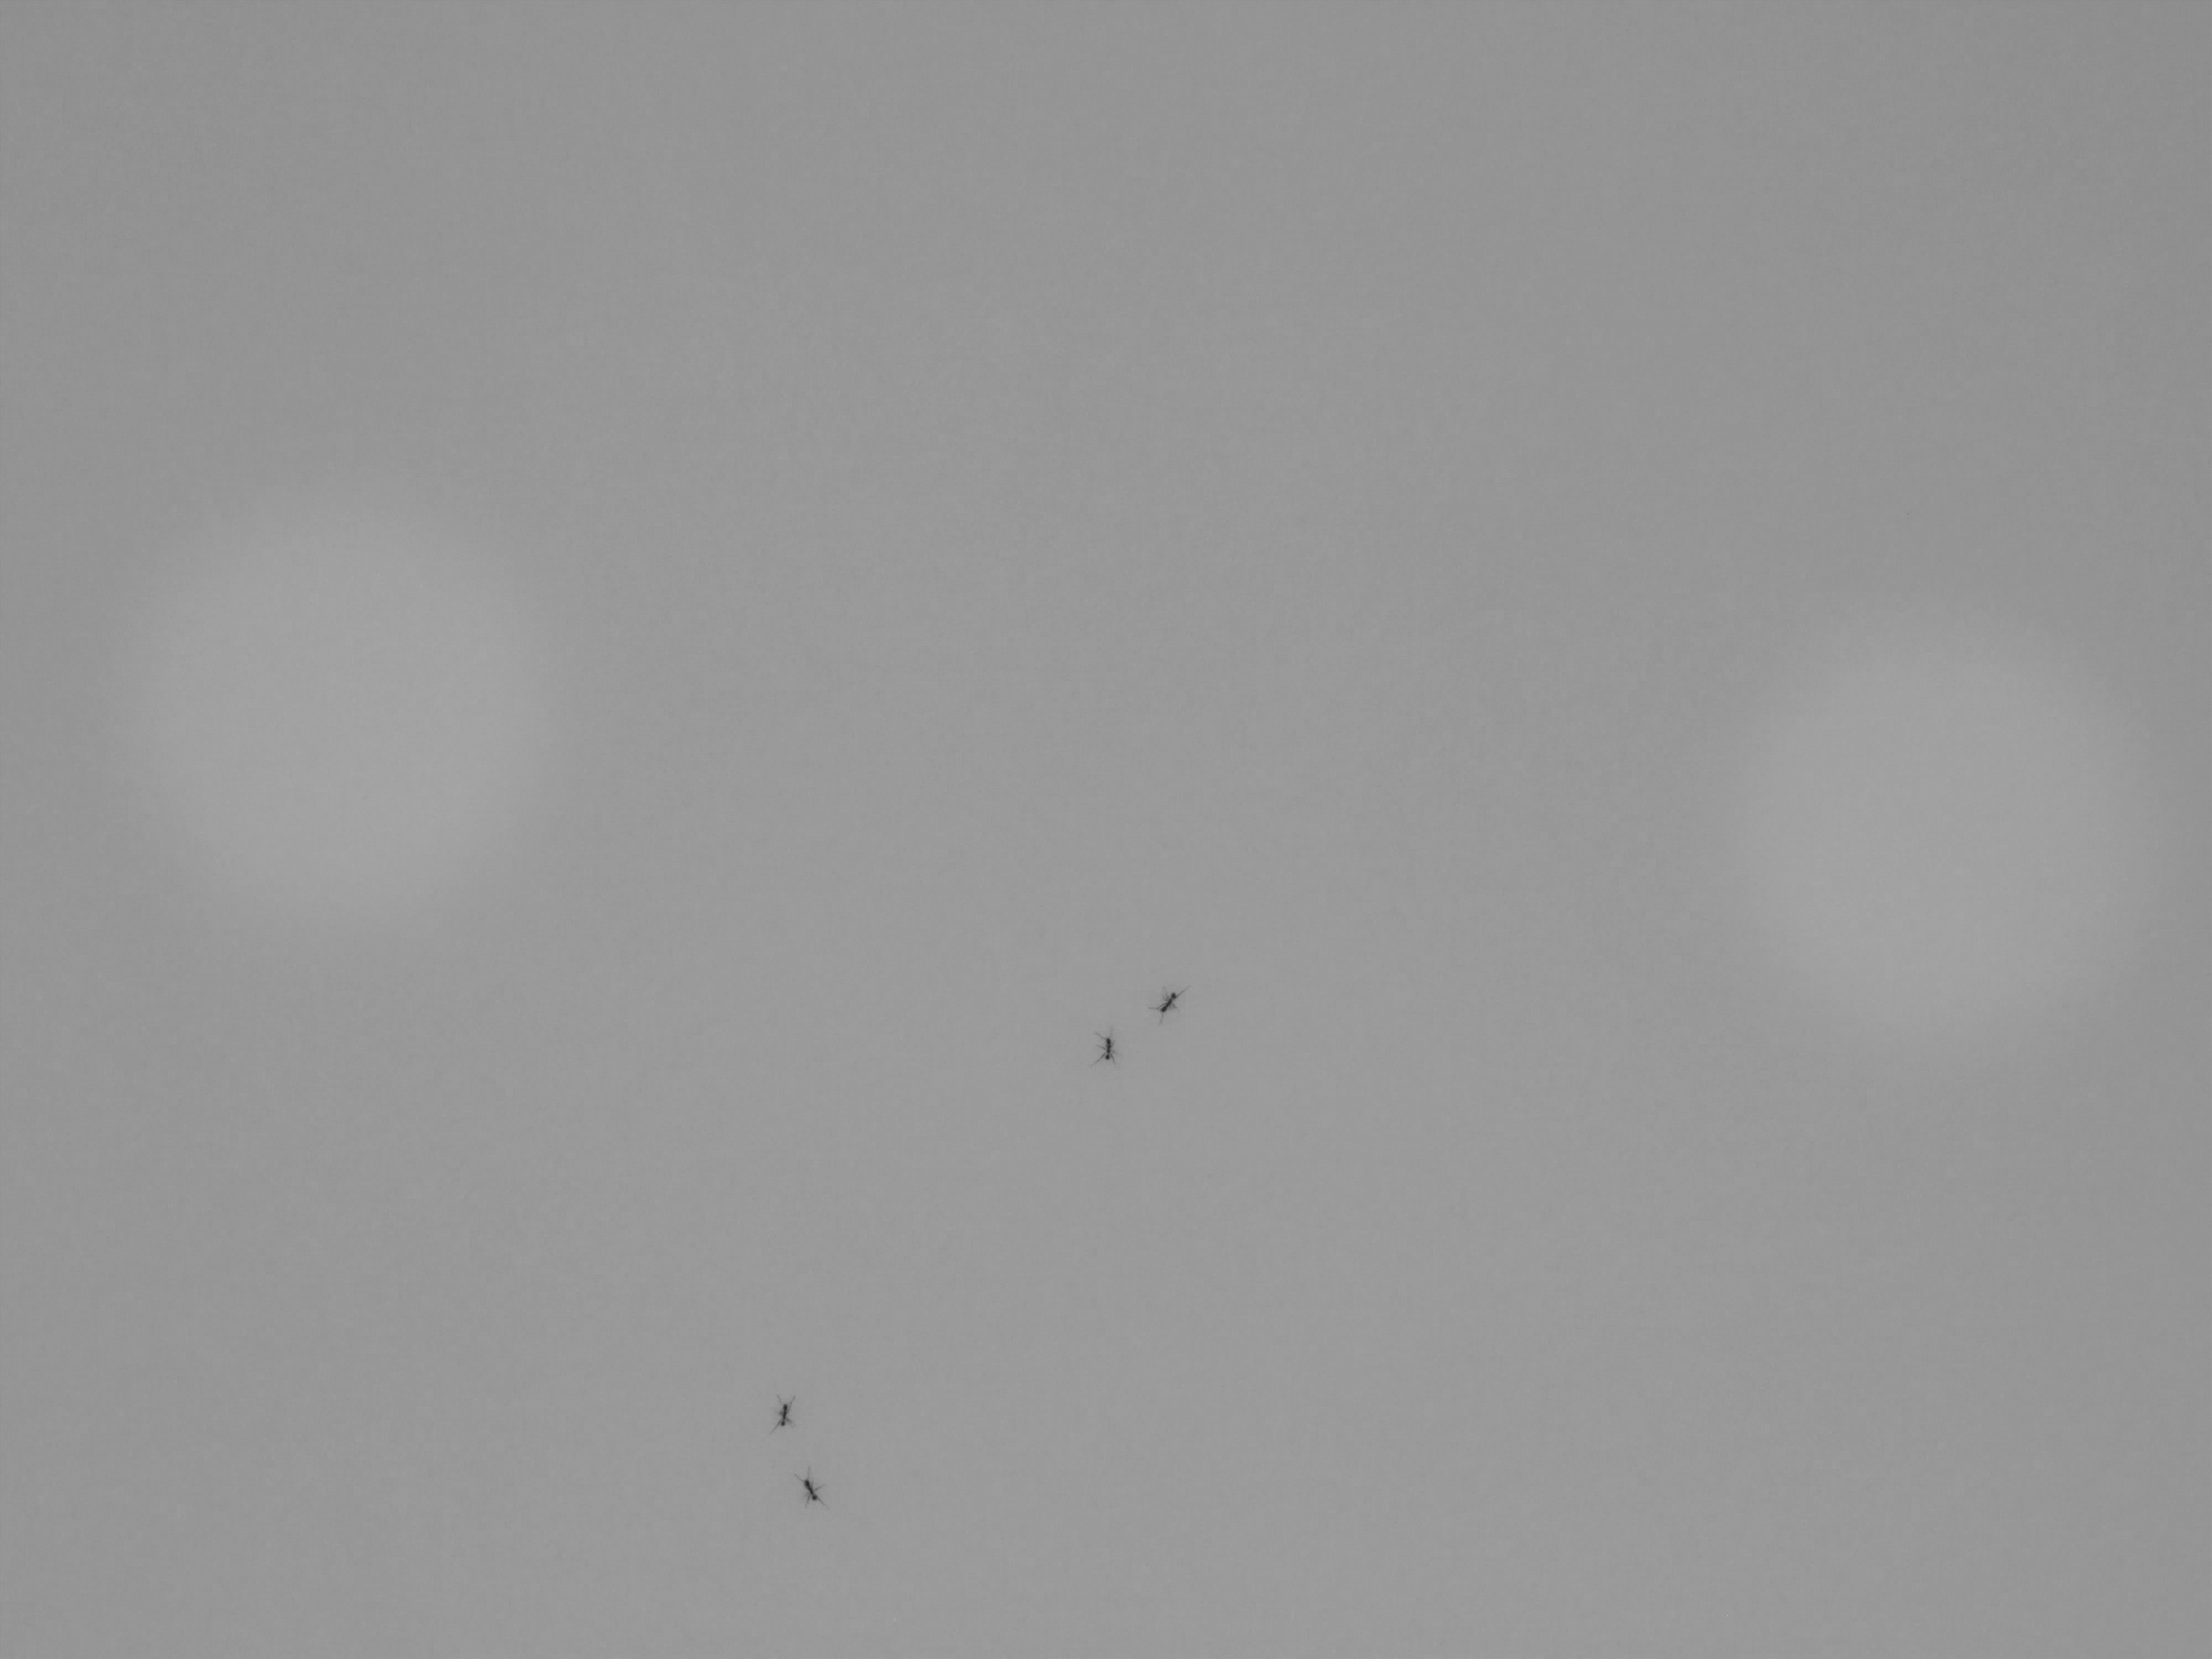
\includegraphics[width=\linewidth]{figures/05_methodology/initial_video_full.png}
        \caption[Frame from the initial video]{\footnotesize{A frame from the initial video.}}
        \label{fig:full frame initial video}
    \end{subfigure}
    \hspace{0.025\linewidth}
    \begin{subfigure}[b]{0.4\linewidth}
        \includegraphics[width=\linewidth]{figures/05_methodology/initial_video_ant.png}
        \caption[Zoom on frame from the initial video]{\footnotesize{A crop from the initial video.}}
        \label{fig:zoom frame initial video}
    \end{subfigure}
    \caption[Frame from the initial video setup]{\footnotesize{The Figure \ref{fig:zoom frame initial video} exposes the net on the upper layer of the Figure \ref{fig:full frame initial video}.}}
    \label{fig:frame initial video}
\end{figure}

\begin{figure}[!p]
    \centering
    \includegraphics[width=0.4\linewidth]{figures/05_methodology/second_video_full.png}
    \caption[Frame from the appearance video setup]{\footnotesize{A frame from one of the second set of videos.}}
    \label{fig:frame second video}
\end{figure}

\begin{figure}[!p]
    \centering
    \begin{subfigure}[b]{0.4\linewidth}
        \includegraphics[width=\linewidth]{figures/05_methodology/thirds_video_all.png}
        \caption[Frame from the more crowded tray video]{\footnotesize{A frame from the tray video with 87 ants.}}
        \label{fig:frame third video all}
    \end{subfigure}
    \hspace{0.025\linewidth}
    \begin{subfigure}[b]{0.4\linewidth}
        \includegraphics[width=\linewidth]{figures/05_methodology/thirds_video_set.png}
        \caption[Frame from the less crowded tray video]{\footnotesize{A frame from the tray video with 46 ants.}}
        \label{fig:frame third video set}
    \end{subfigure}
    \caption[Frames from the tray videos setup]{\footnotesize{Frames from the tray videos setup.}}
    \label{fig:frame third video}
\end{figure}

\FloatBarrier

\paragraph{MOT Challenge Format}

{
    To make the collected data useful for the tracking system, it must undergo a labeling process. 
    The main annotation format that was used is the \textbf{\ac{MOT} Challenge format}\cite{MOTChallenge2015}, 
    which is well-suited for both object tracking and object detection in videos. 
    This format is implemented as a \ac{CSV} text file per video with each line containing 10 fields: 
}

\begin{center}
    {``Frame, Id, left, top, width, height, confidence, 3D-World x, 3D-World y, 3D-World z"}
\end{center}

{
    In the case of 2D data, the 3D-World values are set to -1 and, in the case of detections, the Id value is also set to -1.
}

%\begin{table}[!h]
%    \centering
%    \caption[MOT Challenge format]{ \footnotesize MOT Challenge format with default values.}
%    \label{tab:MOT Challenge format}
%
%    \begin{tabularx}{\textwidth}{@{\hspace{1em}}Xl@{\hspace{1em}}|@{\hspace{1em}}X@{\hspace{1em}}X@{\hspace{1em}}}
%        \toprule
%        \textbf{Column} & \textbf{Field Name} & \textbf{Detection} & \textbf{Tracking} \\
%        \midrule
%        \midrule
%        1 & Frame number & \textless frame\textgreater & \textless frame\textgreater \\
%        2 & Identity number & -1 & \textless id\textgreater \\
%        3 & Detection left & \textless bb\_left\textgreater & \textless bb\_left\textgreater \\
%        4 & Detection top & \textless bb\_top\textgreater & \textless bb\_top\textgreater \\
%        5 & Detection width & \textless bb\_width\textgreater & \textless bb\_width\textgreater \\
%        6 & Detection height & \textless bb\_height\textgreater & \textless bb\_height\textgreater \\ 
%        7 & Detection confidence & \textless conf\textgreater & \textless conf\textgreater \\
%        8 & 3D World x & -1 & -1 \\
%        9 & 3D World y & -1 & -1 \\
%        10 & 3D World z & -1 & -1 \\
%        \bottomrule
%    \end{tabularx}
%
%\end{table}


{
    In addition to the main \ac{MOT} format, this project employs various dataset formats to simplify the training and deployment of different models. 
    These formats include the \ac{YOLO} dataset format\cite{yoloFormat} for image object detection, 
    the Market-1501 dataset format\cite{Market-1501} for appearance modeling, 
    and a custom format tailored for segmenting valid frames and IDs from the appearance videos.
}

\paragraph{YOLO Format}

{
    The \ac{YOLO} format is utilized for labeling single images extracted from videos. 
    Each image is associated with an equally named \ac{CSV} text-file that contains the following column fields for each detection:
}

\begin{center}
    {``class id, x-axis center, y-axis center, width, height"}
\end{center}

{
    It's important to note that the image fields are normalized based on the image shape. 
    Additionally, the \ac{YOLO} format defines a specific folder structure that separates images and labels into subfolders stemming from the same root. 
    A YAML file is used to describe the data paths and class indexes for each dataset.
}

{
    A tool was developed to convert the videos with a MOT Challenge annotations into images with a valid \ac{YOLO} format dataset. 
    This tool offers the flexibility to crop images (and the corresponding labels) into different segments, ensuring that each segment contains at least one whole ant in a random position. 
    The cropping feature maximizing the number of whole ants within each crop while guaranteeing that each ant is fully visible in at least one crop.
    Figure \ref{fig:yolo crop} shows an example of the results of this tool on a video.
}

\begin{figure}[!b]
    \centering
    \includegraphics[width=0.4\linewidth]{figures/05_methodology/yolo_crop.png}
    \caption[YOLO dataset: crop of 640x640 px]{\footnotesize{A crop of 640x640 px generated from an annotated video to create a YOLO Dataset.}}
    \label{fig:yolo crop}
    \vspace{-3em}
\end{figure}

\FloatBarrier

\begin{figure}[!htp]
    \centering
    \begin{subfigure}[b]{0.4\linewidth}
        \includegraphics[width=\linewidth]{figures/05_methodology/Market_unoriented.png}
        \caption[Samples of the unoriented appearance dataset]{\footnotesize{35 samples of the unoriented appearance dataset.}}
        \label{fig:unoriented appearance}
    \end{subfigure}
    \hspace{0.025\linewidth}
    \begin{subfigure}[b]{0.4\linewidth}
        \includegraphics[width=\linewidth]{figures/05_methodology/Market_oriented.png}
        \caption[Samples of the oriented appearance dataset]{\footnotesize{35 samples of the oriented appearance dataset.}}
        \label{fig:oriented appearance}
    \end{subfigure}
    \caption[Samples of the appearance datasets]{\footnotesize{Comparison between the output of the oriented and unoriented versions of the appearance dataset generation tools.}}
    \label{fig:appearance dataset}
    \vspace{-1.5em}
\end{figure}

\paragraph{Market-1501 Format}

{
    Market-1501 is a widely-used reidentification dataset organized based on folder and filename structures. 
    In this project, we mimic this format to simplify the deployment of the appearance model training, we call it Market-1501 Format.
}

{
    In Market-1501 Format, each ``ground truth detection" is cropped from the video and saved as an image within one of three folders: train, test, or test query. 
    and contains its identity on the filename. The identity of each detection is encoded in the filename.
}

{
    To convert the videos with MOT Challenge annotations into a Market-1501 dataset, a pair of tools were developed. 
    The first tool generates square crops using one of three strategies: 
    ``cropping and padding", ``cropping, padding the small size, and reshaping", or ``cropping and reshaping".
    The second tool generates rectangular crops with the head of the ant pointing downwards; 
    the shape of the crop is adjusted using similar methods to those employed by the first tool, 
    with the "padding the small size" option in the second tool being replaced by "padding to obtain the correct aspect ratio."
}

{
    The process of orienting the head of the ant downwards involves four steps:
}

\enlargethispage{1.5\baselineskip}

\begin{enumerate}
    \item The segmentation of the cropped ant by thresholding\footnote{Thresholding (neologism): Act of splitting a set of values using a threshold value.} the luminance level of the image.
    \item The computation of the direction of the body of the ant through principal component analysis.
    \item Determining the movement direction of the ant by comparing the current frame position with the nearest frame were the ants appears (if it is a previous frame, the origin point is the previous frame).
    \item Selecting the body direction of the ant that minimize the angular difference with the movement direction.
\end{enumerate}

\needspace{0.2\textheight}

{
    Figure \ref{fig:appearance dataset} provides an example of the output from each tool. 
    In both cases, padding was applied to one side before reshaping the crop.
    While there is an improvement, it's worth noting that the orientation solution in Figure \ref{fig:oriented appearance} has some limitations, 
    with a total of 35 instances, including 17 correct cases, 15 upside-down cases, and 3 instances with incorrect orientation.
}

\FloatBarrier

\paragraph{Custom Format}

{
    The custom format for segmenting video fragments is structured as a \ac{TSV} file with three columns. 
    The first column indicates the initial frame number, 
    the second column indicates the final frame number, 
    and the last column comprises a Python-styled list of lists that represents the invalid intervals. 
    These intervals are encoded by specifying their initial and final frames.
}

{
    Labeling is a time-consuming task that necessitates human supervision. 
    To reduce the time required, we employed an existing application and developed three additional tools.  
    The research on data annotation was conducted concurrently with the creation of a tutorial designed to guide the annotation of new training videos, which was one of the project's objectives.
}

\needspace{0.2\textheight}

\subsubsection{CVAT}

{
    \ac{CVAT}\cite{cvat} is an interactive annotation tool designed for computer vision applications. 
    It provides support for importing and exporting annotations in various popular formats. 
    In this project, we primarily relied on tracking results for labeling to save time on the annotation process.
}

{
    To set up \ac{CVAT}, it should be installed as a server through their Docker image and accessed through any web browser. 
    Figure \ref{fig:CVAT} shows the annotation interface.
}

{
    \ac{CVAT} manage each id as a class. 
    Within a frame, it offers functionalities to create, delete, and modify detections. 
    Additionally, any track can be created, deleted, marked as finished, split, merged, or have its identity changed.
    For unfinished tracks with gaps in the annotations, \ac{CVAT} employs linear interpolation, which can be adjusted manually in the desired frames.
}

{
    One limitation of \ac{CVAT} is that it supports a maximum resolution of 3000x2000 pixels.  
    To work around this, we utilized ffmpeg\cite{tomar2006converting} to downsample the video file and developed two scripts to adapt the annotations accordingly. 
    The commands in Listing \ref{lst:cvat_input} are used to generate the input video and importable annotations.
}

\begin{footnotesize}
    \begin{bashcode}[float=h, label={lst:cvat_input}, language=bash, caption={Commands to obtain the CVAT compatible data}]
        ffmpeg -y -i input.mp4 -vf scale=2000:-2,setsar=1:1 -c:v libx264 "input_downsampled.mp4"
        python3 minimum_id.py input_1.txt input_2.txt
        python3 prde_to_cvat.py input_2.txt output.zip
    \end{bashcode}
\end{footnotesize}

{
    A script was also created to convert manually corrected but downsampled annotations into the desired resolution.
}

{
    Despite the availability of preannotations from tracking models and the utility of this tool, 
    annotating 1375 frames (equivalent to approximately 1 hour and 30 minutes of video) still requires around 2 hours.
}

\begin{figure}[!tp]
    \centering
    \includegraphics[width=0.7\linewidth]{figures/05_methodology/CVAT.png}
    \caption[CVAT interface]{\footnotesize{A screenshot of the CVAT interface.}}
    \label{fig:CVAT}
\end{figure}

\subsubsection{Lonely Ant Frame Segmentation}

{
    In the process of generating video segment annotations from the collection of videos for appearance training, 
    a text file is filled manually with the previously listed specifications. 
    To speed up the process, a command that write the frame number on each frame using the ffmpeg tool is employed, as illustrated in Listing \ref{lst:frame_num_video}:
}

\begin{footnotesize}
    \begin{bashcode}[float=!h, label={lst:frame_num_video}, language=bash, caption={Command to write the frame number on each frame}]
        ffmpeg -i input.mp4 -vf "drawtext=fontfile=Arial.ttf: text=%{n}: fontsize=24: x=(w-tw)/2: y=h-(2*lh): fontcolor=white@0.5: box=1:boxcolor=0x00000099@0.3" -y input_frame_num.mp4
    \end{bashcode}
\end{footnotesize}
\FloatBarrier

{
    This approach reduces the time required for annotation to approximately 15 minutes for every hour of video footage. 
    Note that a video can be played at an accelerated speed, and this annotations only require pausing the video.
}

{
    Moreover, when dealing with sequences involving only one ant per frame and employing a high-performance detector, 
    this method becomes analogous to annotating in the MOT Challenge format. 
    By utilizing \textbf{detection by tracking}, the detector can effectively allow the low-confidence detections\footnote{This improves the detection recall, recall is a metric that will be explained in the following subsection about metrics.} and utilize a tracker to eliminate false positives.
    Even if the detector does not eliminate all the false positives, 
    adhering to the strict criterion of one ant per frame enables the initial exclusion of frames featuring multiple ants, 
    which can subsequently be interpolated as required.
}

\subsubsection{Purging by Deletion}

{
    A reliable object detector relies on a clean object detection dataset. 
    Given the impracticality on annotating with \ac{CVAT}, a different approach to create a object detection dataset was designed.
    This process utilized the script previously explained for generating a cropped (or uncropped) YOLO dataset, as illustrated in Figure \ref{fig:yolo crop}.
    To accomplish this, two additional scripts were developed.
}

{
    The initial step involves generating the object detection dataset using the YOLO dataset script. 
    The image filenames are assigned based on the frame IDs 
    (if no cropping was applied, it can be easily transformed into the MOT format).
}

{
    Next, the second script comes into play, which annotates the images and saves them in a new folder. 
    In cases where only one detection exists, a crop is retained, as it simplifies the process of assessing its accuracy via a file explorer. 
}

{
    Subsequently, annotators are tasked with deleting the invalid images from this folder.
}

{
    In the final step, a script is employed to construct a new dataset by copying only the remaining images. 
    This results in an object detection dataset where only a fraction of the frames are preserved, 
    typically less than half of the images prove to be valid.
}

{
    As an example, 50 seconds (equivalent to 750 frames) are transformed into 13,000 crops, 
    equivalent to a duration of approximately 14 minutes and 27 seconds. 
    The annotation process for this sequence typically takes around 4 hours to complete.
}

\subsubsection{Cleaning by Crop Deletion}

{
    While discarding images containing errors is an acceptable practice for object detection datasets, the aim is often to maximize available data. 
    To address this, we implemented another set of scripts, similar to the ones described previously.
}

{
    In this scenario, the data is initially in MOT format both at the beginning and the end of the process. 
    The first script is designed to store cropped images alongside their corresponding frame IDs and line numbers.  
    This script can source data from either one or two models. 
    In cases involving two models, it combines their outputs and attempts to identify true positives (which can be reviewed more swiftly), false positives, and false negatives.  
}

{
    The second script generates a MOT format file containing only the remaining lines, meaning that annotations for frames are corrected rather than deleted.
}

{
    In this case, cleaning 1 hour of video containing a single ant (equivalent to 54,000 frames) can be accomplished in roughly 6 hours. 
    This process was applied to 9 out of the 12 individual ant videos.
}

\needspace{0.2\textheight}

\subsubsection{Labeling strategies summary}

{
    The following table shows the speed of each strategy:
}

\begin{table}[H]
    \centering
    \caption[Labeling strategies speed]{ \footnotesize Labeling strategies speed }
    \label{tab:labeling speed}

    \begin{tabularx}{0.7\textwidth}{
        @{\hspace{0.05\textwidth}}
        >{\raggedright\arraybackslash}X
        >{\raggedleft\arraybackslash}X
        @{\hspace{0.05\textwidth}}
    }
        \toprule
        \textbf{Strategy} & \textbf{Speed} \\
        \midrule
        \midrule
        CVAT & 0.2 fps \\
        Lonely ant frames & 60 fps \\
        Purging by deletion & 0.9 fps \\
        Cleaning by deletion & 2.5 fps \\
        \bottomrule
    \end{tabularx}
\end{table}

\FloatBarrier

\needspace{0.25\textheight}
\subsection{Metrics}


{
    In the development of any engineering system, a fundamental aspect is the measurement of its performance. 
    In this project, we have one primary system, the \ac{MOT} tracker, along with two subsystems: the object detector and the appearance model. 
    Each of these components has its own set of evaluation metrics to quantify its performance
}

\subsubsection{Object Detection Metrics}

{
    An object detector solves the object localization and classification problems at the same time. 
    This kind of problem is evaluated by the precision, recall, F1-Score and \ac{mAP} metrics.
}

{
    These metrics require the definition of true positives, false positives and false negatives:
}

\begin{itemize}
    \item The \textbf{true positives} (\acs{TP}) are defined by correctly matching a class detections with ground truth objects of the same class. Usually a \ac{IoU} threshold is used to match the detections, similar to the association step of a SORT tracker.
    \item The \textbf{false positives} (\acs{FP}) are defined by incorrectly assigning a class on the detected object, it applies to matched objects and detected background.
    \item The \textbf{false negatives} (\acs{FN}) are defined by the absence of matching detections for ground truth objects.
\end{itemize}

\paragraph{Precision}

{
    Precision is a metric that measures the correctness of the detected set, a high precision means a high certainty on the detected objects, however it does not contemplate undetected objects.
}

\paragraph{Recall}

{
    Recall is a metric that measures the ability to detect targets, a high recall means a high certainty on detecting the relevant objects, however it does not contemplate undesired detections.
}

%\begin{figure}[!ht]
%    \centering
%    \includegraphics[width=0.3\linewidth]{figures/05_methodology/Precisionrecall.png}
%    \caption[Precision and recall]{\footnotesize{Visual representation of precision and recall extracted from WikipediaCommons\cite{precision_recall}.}}
%    \label{fig:precision and recall}
%\end{figure}
%
%{
%    Figure \ref{fig:precision and recall} describes graphically and mathematically precision and recall.
%}

\paragraph{F1-Score}

{
    F1-Score is the harmonic mean of precision and recall which symmetrically represents both metrics, it allows a good global evaluation of a model. 
%    Its formula is the following:
}

%\begin{equation}
%    \label{eqn:F1Score}
%    F_{1} = 2 \cdot \frac{precision \cdot recall}{precision + recall}
%\end{equation}

%{
%    Usually, deep learning based detection models return their confidence score. 
%    F1-Score, precision and recall computed on a validation dataset can be used to determine that parameter.
%    There is a compromise between precision and recall that makes the choice of a good threshold a non-trivial task.
%}

\paragraph{Mean Average Precision}

{
    \ac{AP} and \acl{mAP} (\ac{mAP}) are other global performance metrics like F1-Score. 
    \ac{AP} join precision and recall regardless of the confidence threshold for a given class. 
    \Ac{mAP} averages the \ac{AP} metric across multiple outputs generated by various user-defined settings. 
    These sets of outputs are referred to as queries.
}

{
    The most popular conventions for the \ac{mAP} set of settings are the isolation of each class and the definition of multiple \ac{IoU} threshold used to match the detections with the ground truth. 
    This project only detects one class, which means that only the \ac{IoU} threshold is modified.
}

%{
%    The \ac{AP} metric is obtained by averaging the precision curve ($P(R)$) in function of the recall ($R$) from 0 to 1:
%}

%\begin{equation}
%    \label{eqn:AP theory}
%    AP = \int_{0}^{1} P(R) \, dR
%\end{equation}

%{
%    In practice, the precision and recall curve is estimated by a given dataset becoming a set of not equidistributed points. 
%    In order to average the precision and recall curve, the data output is sorted by decreasing confidence (the $i-th$ detection is ranked $k_{i}$), the precision is computed within a subset of the $k$ more confident detections ($P(k)$) and, at the end, each ranked precision is weighted averaged by the width of the recall interval from the previous rank to the current rank.
%}

%\needspace{0.1\textheight}

{
%    The mathematical expression of the defined weighted average can be simplified into the simple mean of the ranked precision of the ground truth elements, with the false negatives redefined to have a ranked precision of 0:
    The \ac{AP} metric is obtained by averaging the precision in function of the recall curve. In practice, an estimation is obtained by a weighted average that can be simplified into the simple mean of the ranked precision of the ground truth elements, with the false negatives redefined to have a ranked precision of 0:
}

\begin{equation}
    \label{eqn:AP real}
    AP = \frac{\mathlarger{\sum\limits_{i \in TP}} P(k_{i})}{|TP| + |FN|}
\end{equation}

{
    This project uses the \textbf{\ac{mAP}@50} (or \ac{AP}@50 because there is only one class) and the \textbf{\ac{mAP}@50-95}. 
    The @ notation refers to the \ac{IoU} threshold queries, being \textbf{\ac{mAP}@50} the \ac{AP} when the \ac{IoU} is set to 0.5 and \textbf{\ac{mAP}@50-95} the mean of the \ac{AP} computed with \ac{IoU} thresholds of 0.5, 0.55, 0.6, 0.65, 0.7, 0.75, 0.8, 0.85, 0.9 and 0.95.
}

\subsubsection{Identity Re-identification Metrics}

{
    An appearance model solves the identity re-identification problem. 
    This kind of problem is evaluated by the rank metrics and the already seen \textbf{\ac{mAP}} using the identities on the desired validation dataset classes as queries.
}

{
    In re-identification problems true negatives can also be defined, in addition to true positives, false positives and false negatives:
}

\begin{itemize}
    \item The \textbf{true positives} are defined by correctly matching pairs of ants images with the same identity.
    \item The \textbf{true negatives} (\acs{TN}) are defined by correctly not matching pairs of ants images with different identities.
    \item The \textbf{false positives} are defined by incorrectly matching pairs of ants images with different identities.
    \item The \textbf{false negatives} are defined by incorrectly not matching pairs of ants images with the same identities.
\end{itemize}

\paragraph{Rank metrics}

{
    The $k$-rank metrics redefine true positives (${TP}_{k}$) by the existence on any correct match for a query ant within the $k$ nearest appearances.
    The final metric is the accuracy of the given set of queries:
}

\begin{equation}
    \label{eqn:rank accuracy}
    Rank_{k} = \frac{|{TP}_{k}|}{|queries|}
\end{equation}

{
    This project contemplates the rank-1 metric or accuracy.
}

\needspace{0.15\textheight}

\subsubsection{Multiple Object Tracking Metrics}

{
    Evaluating multiple object tracking is a complex problem comparable to the tracking task itself. 
    The reason of this complexity is the fact that a tracking system solves 3 problems:
}

\begin{itemize}
    \item \textbf{Detection}: the target objects are found. % independently of the identity. but the matching score priorize identity to get TP anyway
    \item \textbf{Localization}: the found objects are spatially aligned with their target. % independently of the identity. but the matching score priorize identity to get TP anyway
    \item \textbf{Association}: the found objects are temporally aligned with their target identity.
\end{itemize}

{
    For this reason, there exist a lot of metrics that prioritize one problem over the others or evaluate each problem with different criteria.
    In this project, it was decided to use the \ac{HOTA}\cite{luiten2020IJCV} group of metrics because the authors of these metrics states that the \ac{HOTA} metric, that jointly evaluates the three problems, is balanced with respect the three problems (see Figure \ref{fig:hota_vs_others}).
}

\begin{figure}[!h]
    \centering
    \includegraphics[width=0.75\linewidth]{figures/05_methodology/HOTA_vs_other.png}
    \caption[HOTA compared with other metrics]{\footnotesize{
        Image extracted from the HOTA paper\cite{luiten2020IJCV}. \\
        HOTA, DetA and AssA compared with other popular metrics (MOTA\cite{MOTA} and IDF1\cite{ristani2016performance}).
        }}
    \label{fig:hota_vs_others}
\end{figure}

{
    Similar to the other metrics, the first step is the definition of true positives, false negatives and false positives. 
    However, to obtain these values, a matching between ground truth and tracks is required.
    This matching should aim to maximize the final metric while maintaining plausibility. 
    The rationale behind this criterion is that all consistent interpretations of the system's output that align with the ground truth are valid, 
    and the maximized interpretation is likely the most accurate.
}

{
    The authors of \ac{HOTA} solve this optimization problem with the Hungarian algorithm using a composed score. The score uses a \textbf{current frame} spatial similarity component and a \textbf{global} estimated ``optimal association" score.
    The estimated association score is a prematching proxy for an association score that approaches the estimated one for the optimal assignment.
}

{
    The spatial similarity can be the previously explained \ac{IoU}, the previous ``plausibility'' refers to a threshold value applied on this score after the ground truth matching. 
}

{
    The estimated association score is a multiple frames Jaccard index\footnote{The Jaccard index is the intersection of two sets over their union (\ac{IoU}).}, it is computed as the available spatial associations (with a higher spatial similarity than the threshold) of a pair ``ground truth identity''-``tracked object identity'' for all the frames over the number of frames where at least one of the identities was present (see Figure \ref{fig:hota_preassociation}).
}

\begin{figure}[!h]
    \centering
    \includegraphics[width=\linewidth]{figures/05_methodology/HOTA_association_example.png}
    \caption[HOTA: Track overlap with ground truth]{\footnotesize{
        This image illustrates a case where a track of 3 frames overlaps during 2 frames with a ground truth identity of 4 frames. 
        The denominator of the estimated optimal association will be 3-2+4=5. 
        The numerator can be 2 for a threshold smaller than 0.5, 1 for a threshold smaller than 0.8 and 0 for a threshold higher than 0.8. 
        With a threshold of 1 the association score cannot be different than the estimated association score.
        }}
    \label{fig:hota_preassociation}
\end{figure}

{
    Once the spatial similarity ($\mathcal{S}$), the estimated association score ($\mathcal{A}_{max}$) and the similarity threshold ($\alpha$) are defined, the potential matching score used for the linear assignment joins them as in the equation \ref{eqn:potential matching score}:
}

\begin{equation}
    \label{eqn:potential matching score}
    MS(i, j) = \begin{cases}
        \frac{1}{\varepsilon} + \mathcal{A}_{max}(i, j) + \varepsilon \cdot \mathcal{S}(i, j) & \text{if } \mathcal{S}(i, j) \geq \alpha\\
        0 & \text{otherwise}
    \end{cases}
\end{equation}
    
{
    The matching algorithm was implemented in order to use the ground truth to analyses our results and test the viability of a model.
}

{
    With a mapping between ground truth and output tracks, \ac{HOTA} defines true positives, false negatives, false positives:
}

\begin{itemize}
    \item The \textbf{true positives} are detections that are matched with a ground truth object, independently of the identity, it measures the performance of the detection and localization problems.
    \item The \textbf{false negatives} are ground truth objects that are not matched.
    \item The \textbf{false positives} are detections that are not matched.
\end{itemize}

{
    Additionally, \ac{HOTA} defines new values called true positives associations (\acs{TPA}), false negatives associations (\acs{FNA}) and false positives associations (\acs{FPA}).
    The \ac{TPA}, \ac{FNA} and \ac{FPA} are defined independently over all the pairs of ``ground truth identity''-``tracked object identity'' within the true positives set; a single evaluation has got one set of true positives, false negatives and false positives and $C=|TP|$ sets of true positives associations, false negatives associations and false positives associations. 
    These values measure the performance of the association problem:
}
\begin{samepage}
    \begin{itemize}
        \item The \textbf{true positives associations}, given a true positive of interest ``c", are all the true positives which have the same ``ground truth identity''-``tracked object identity'' pairs than the interest true positive ``c"; all \ac{TPA}s have the same \ac{TPA}, \ac{FNA} and \ac{FPA} which reduce the number of computation although the concept is defined for all the \ac{TP}s.
        \item The \textbf{false negatives associations}, given a true positive of interest ``c", are the ground truth objects with the same identity as the ground truth from ``c'' that were not assigned the tracked object identity from ``c'' (different or unassigned identities).
        \item The \textbf{false positives associations}, given a true positive of interest ``c", are the detections with the same identity as the detection from ``c'' that were not assigned the ground truth identity from ``c'' (different or unassigned identities).
    \end{itemize}
\end{samepage}

{
    With the new association measures, the previously mentioned association score can be properly defined:
}

\begin{equation}
    \label{eqn:association score}
    \mathcal{A}(C) = \frac{|TPA(c)|}{|TPA(c)| + |FNA(c)| + |FPA(c)|}
\end{equation}

\paragraph{\ac{HOTA}\textsubscript{$\alpha$}}

{
    \ac{HOTA}\textsubscript{$\alpha$} is a metric defined by a double Jaccard formulation, where the association score ($\mathcal{A}$) is a Jaccard metric over the associations that weights the true positives of a Jaccard metric over the detection concept. 
    And $\alpha$ is the threshold on location similarity.
}

\begin{equation}
    \label{eqn:hota alpha}
    HOTA_{\alpha} = \sqrt{\frac{\sum_{c \in \{TP\}} \mathcal{A}(c)}{|TP| + |FN| + |FP|}}
\end{equation}

{
    The square root is needed because the dimensionality of the summation of association scores (multiplied by true positive of value 1) is squared (jointly detection domain and association domain) over unsquared (association domain), and the detection Jaccard makes the denominator squared (jointly detection domain and association domain).
}

\paragraph{\ac{HOTA}}

{
    Theoretically, \ac{HOTA} is the average of $HOTA_{\alpha}$ on all the location similarity domain (from 0 to 1). In practice, it can be approximated by a mean:
}

\begin{equation}
    \label{eqn:hota}
    \text{HOTA} = \int_{0}^{1} \text{HOTA}_{\alpha} \, d\alpha \approx \frac{1}{19} \cdot \sum_{\alpha \, \in \, \{0.05 \cdot i \,|\, 1 \leq i \leq 19\}} \text{HOTA}_{\alpha}
\end{equation}

\paragraph{LocA}

{
    Localization Accuracy (\ac{LocA}) is a measure of localization that average the different localization thresholds:
}

\begin{equation}
    \label{eqn:loca}
    \text{LocA} = \int_{0}^{1} \frac{1}{|\text{TP}_{\alpha}|} \cdot \sum_{c \, \in \, \{\text{TP}_{\alpha}\}} \mathcal{S}(c) \, d\alpha
\end{equation}

\paragraph{DetA}

{
    Detection Accuracy (\ac{DetA}) is the detection Jaccard index with a given localization threshold $\alpha$. It can be further decomposed into detection precision and detection recall but it is not used in this project.
}

\begin{equation}
    \label{eqn:deta}
    \text{DetA}_{\alpha} = \frac{|\text{TP}_{\alpha}|}{|\text{TP}_{\alpha}| + |\text{FN}_{\alpha}| + |\text{FP}_{\alpha}|}
\end{equation}

\paragraph{AssA}

{
    Association Accuracy (\ac{AssA}) is a measure of association that average the association score with a given localization threshold $\alpha$.
}

\begin{equation}
    \label{eqn:assa}
    \text{AssA}_{\alpha} = \frac{1}{|\text{TP}_{\alpha}|} \cdot \sum_{c \, \in \, \{\text{TP}_{\alpha}\}} \mathcal{A}(c) \, d\alpha
\end{equation}

{
    Another interpretation of \ac{HOTA}\textsubscript{$\alpha$} is the geometric mean of \ac{DetA}\textsubscript{$\alpha$} and \ac{AssA}\textsubscript{$\alpha$}.
}


\needspace{0.25\textheight}
\subsection{Detection Models}


{
    To facilitate the development of multiple detection models and their subsequent integration into the tracker, we designed a versatile program. 
    This program processes input videos and saves the output detections in a MOT format file with an easily replaceable detector. 
}

%\begin{figure}[!p]
%    \centering
%    \includegraphics[width=0.6\linewidth]{figures/05_methodology/DetectionScript.png}
%    \caption[Generic detection script]{\footnotesize{
%            Block diagram of the detection script.
%        }}
%    \label{fig:DetectionScript}
%\end{figure}

{
    Initially, there was no labeled data to train any data-driven model, for this reason, the first implemented model was a deductive model.
}

{
    This deductive model, as the examples from the tracking software subsection of the state of the art, is based on background extraction.
}

{
    To ensure accurate background estimation, this model requires a set of training frames. 
    The estimation is performed using a Gaussian Mixture-based model, which becomes reliable after proper training. 
    In this project, 500 frames were used because the input videos allowed it, however, with 50 frames is enough.
}

{
    Once the background is estimated, it is subtracted from the frame to isolate the foreground. 
    A morphological filter consisting in a 5x5 closure to reduce noise inside the ant body, 
    followed by a 3x3 opening is then applied to the foreground to reduce noise in the background estiamtion. 
    The remaining connected components with a minimum pixel count are identified as the output detections.
}

%\begin{figure}[!h]
%    \centering
%    \includegraphics[width=0.6\linewidth]{figures/05_methodology/fgbg_code.png}
%    \caption[Background extraction detection model block diagram]{\footnotesize{
%            Block diagram of the background extraction based model.
%        }}
%    \label{fig:fgbg_code}
%\end{figure}

\FloatBarrier

{
    With the first detection model results, filtered by a tracker and corrected with the developed annotation tools, a initial dataset was created; it was used to train a deep learning model.
    After some iterations of training, detection of new data and cleaning, the final dataset used for detection training was created. 
    The test was performed on an unseen set of data manually annotated: a video fragment which can represent the final deployment.
    The first video was excluded.
}

{
    The following table contains the training, validation and test splits:
}

\begin{table}[H]
    \centering
    \caption[Detection dataset size]{ \footnotesize Detection dataset size.}
    \label{tab:detection splits}

    \begin{tabular}{p{3cm} rr}
        \toprule
        \textbf{Subset} & \textbf{Images} & \textbf{Percentage} \\
        \midrule
        \midrule
        \textbf{Training} & 8374 & 68.7\% \\
        \textbf{validation} & 3662 & 30.1\% \\
        \textbf{Test} & 150 & 1.2\% \\
        \bottomrule
    \end{tabular}
\end{table}

{
    The deep learning model selected for this project is the Ultralytics\cite{Jocher_YOLO_by_Ultralytics_2023} library \ac{YOLOv8} architecture \ac{YOLOv8n} model (detailed in the state of the art section).
    The decision to opt for this architecture was based on state of the art performance in popular challenges as well as simplicity of training and inference deploying (Ultralytics implements most of the standard training features).
}

{
    The choice of model was based on the current problem, the ants on the frames are small objects, and it has two main consequences: 
}

\begin{itemize}
    \item Deep neural networks tend to reduce the spatial dimension while expanding the feature dimension; this means that the ant location becomes uncertain.
    \item Deep neural networks requires a fixed input size, if the input is large, the training may suffer from lack of memory; however, if the input is resized into a smaller size, the small ants may disappear.
\end{itemize}

{
    A slicing windows analysis was deployed in order to solve this issues.
    For the training, 640x640 px crops were used; and, for the inference, a slicing windows was applied using the \ac{SAHI} library\cite{Akyon_Slicing_Aided_Hyper_2022,obss2021sahi}. 
    This method divides the image into a set of overlapped sub-images without any reshaping. 
    However, it results in longer training and inference times, as each image is transformed into multiple sub-images.
}

{
    Additionally, \ac{YOLOv8n}, the smallest \ac{YOLOv8} model, was selected by experimentation.
}

\needspace{0.2\textheight}

\subsubsection{YOLOv8 Training}

{
    Ultralytics is fully integrated with \ac{WandB}\cite{wandb}, a machine learning development platform that helps in the real-time tracking and visualization of experiments, it also have an automatized launcher for hyperparameter sweeping. 
    Using \ac{WandB} resources to visualize enough trainings, the lower and upper thresholds of each available hyperparameter were adjusted until the setting in Table \ref{tab:detection hyperparameters}.
}

\begin{table}[H]
    \centering
    \caption[Detection Model hyperparameters]{ \footnotesize Detection Model hyperparameters.}
    \label{tab:detection hyperparameters}

    \begin{tabularx}{0.9\textwidth}{
        @{\hspace{0.025\textwidth}}
        >{\raggedright\arraybackslash}X
        >{\raggedleft\arraybackslash}X
        @{\hspace{0.025\textwidth}}
    }
        \toprule
        \textbf{Hyperparameter Name} & \textbf{Values} \\
        \midrule
        \midrule
        Hue (maximum deviation) & min=0, max=0.3\\
        Saturation (maximum deviation) & min=0, max=0.5\\
        Value (maximum deviation) & min=0, max=0.5\\
        Rotation (maximum degrees) & min=60º, max=180º\\
        Translation (fraction of input) & min=0, max=0.5\\
        Scale (maximum gain and loss) & min=0, max=1\\
        Flip upside down (probability) & min=0, max=0.5\\
        Flip left-right (probability) & min=0, max=0.5\\
        Mosaic (probability) & min=0, max=1\\
        Shear (maximum degrees) & min=0, max=15\\
        Perspective (fraction) & min=0, max=0.001\\
        Mixup (probability) & min=0, max=0.12\\
        Copy paste (probability) & min=0, max=1\\
        \midrule
        Dropout & \{0, 0.25, 0.5, 0.75\} \\
        \midrule
        Batch size & min=50, max=100 \\
        Optimizer & \{SGD, AdaM\} \\
        Initial learning rate & min=0.001, max=0.01 \\
        Final learning rate & min=0.0001, max=0.001 \\
        Warmup epochs & 10 \\
        Cosine learning rate & \{True, False\} \\
        Momentum & min=0.9, max=0.974 \\
        \midrule
        Maximum epochs & 500 \\
        Early stopping patience & 50 epochs \\
        \midrule
        NMS & \{Agnostic, False\}\\
        NMS IoU & min=0.5, max=1\\
        \bottomrule
    \end{tabularx}
\end{table}

%\needspace{0.25\textheight}

{
    The first group of hyperparameters refer to the data augmentation used to help the model generalize better with the same amount of data, as each time a imaged is loaded, it will be randomly modified within a certain limits. 
    It includes modification in the images coloration, the appearance of the objects within the image, small modifications of the objects (a flip will create a symmetrical but inexistent ant) and some combination of various images. 
    Figure \ref{fig:detector_data_augmentated} shows a set of 16 images after data augmentation.
}

\begin{figure}[!tp]
    \centering
    \includegraphics[width=0.5\textwidth]{figures/05_methodology/TrainDataDetector.jpg}
    \caption[YOLOv8 data augmentated]{\footnotesize{Samples of the augmentated training data for the best detector trained.}}
    \label{fig:detector_data_augmentated}
\end{figure}

{
    The second group of hyperparameters refer to the model, in this case, there is only the dropout; it randomly set to zero certain values in the mathematical expression of a forward pass to reduce the number of useless nodes as well as generalize by randomizing.
}

{
    The third group of hyperparameters refer to the weight upgrading to reach an optimum result on the loss function.
    The loss function for these trainings is a combination of binary cross entropy and focal loss for classification (with only one class, ant, both of them are equivalent) and a mean squared error (\ac{MSE}) for the object location.
    The hyperparameters include the number of images used as a representative sample of the world that the model should learn, how the model will find the best weights to fit the current batch samples and the speed (with not a well-defined meaning) at which it will try to reach that weights.
}

{
    The fourth group set a limit on how long it should take to reach the limit, and the maximum steps admissible without validation improvement.
}

{
    The last group is about post-processing the outputs, only the suppression of highly overlapped detections is contemplated.
}

{
    At the end, the best models were selected, added to the detection script with \ac{SAHI} and their outputs were used in the tracker.
}


\needspace{0.25\textheight}
\subsection{Appearance Model}


{
    Similar to the detection model, the first step was the development of a script that applies the appearance model. 
    In this case, the script takes a MOT format file and its video.
    It applies the appearance model on each line of the MOT file.
    And the output is the input MOT file with each line extended with as many columns as appearance features returns the model.
}

{
    For the appearance model, the choice of model was directly obtained from Deep OC-SORT (a model from 2023): the Bag of Tricks model\cite{Luo_2019_CVPR_Workshops}. 
    The rationale behind this choice was twofold: 
    first, given the limited availability of appearance data, there were modest expectations for its performance in the initial video. 
    Second, Deep OC-SORT represents a state-of-the-art model, further justifying its selection.
}

{
    The implementation of this model is the same from Deep OC-SORT, it is the model from the FastReID\cite{he2020fastreid} library which includes training scripts. 
    In this case, a tuning of the FastReID source code was needed. The inference function was extracted from the Deep OC-SORT code and applied on the developed inference scripts.
}

\subsubsection{Bag of Tricks Training}

{
    Being a relatively simple model architecture (detailed in the state of the art section), 
    the more relevant part of this model is the training, more specifically, the training tricks defined on their paper and code:
}

\begin{itemize}
    \item The triplet loss, a derivable function for maximizing interclass euclidean distance and minimizing intraclass euclidean distance, is applied before the batch normalization layer.
    \item The classification loss is still derivated from the output of the pooling layer.
    \item The first 1000 iterations from a total of 18000 has the backbone freezed.
    \item The first 2000 iterations are warm-up iterations and the learning rate increases.
    \item From the iteration 2000 until the iteration 9000 the learning rate is constant.
    \item From the iteration 9000 until the end, the learning rate decrease with a cosine decay.
\end{itemize}

{
    The implementation used for training is the same of the paper, with the only difference in the data augmentation: the code was modified in order to allow the definition of rotation degrees and the use of rotation without any additional affine transformations. 
    Most of the training options were reduced based on the paper.
}

{
    The biggest ant appearance dataset that was used contained 186 identities, divided into 93 for training and 93 for validating. 
    The validation set will leave a 20\% of the identities as unknown identities (these identities are true negatives). 
    At the end, the train set has got 6730 images, the validation query set has got 489 images to assign in 5795 images. 
}

{
    The model was not tested using the criteria from the training. 
    Nevertheless, a custom set of tests, that will be explained in the following subsection, 
    were performed on an unseen set of data manually annotated: a video fragment with 87 simultaneous identities which represent the worst case scenario.
}

\enlargethispage{1.5\baselineskip}

\needspace{0.1\textheight}

{
    The following table summarize the data splits:
}

\begin{table}[H]
    \centering
    \caption[Appearance dataset size]{ \footnotesize Appearance dataset size.}
    \label{tab:appearance splits}

    \begin{tabular}{p{3cm}l rrr}
        \toprule
        \multicolumn{2}{c}{\textbf{Subset}} & \textbf{Identities} & \textbf{Images} & \textbf{Percentage} \\
        \midrule
        \midrule
        \multicolumn{2}{l}{\textbf{Training}} & 93 & 6730 & 51.1\% \\
        \multirow{2}{*}{\textbf{Validation}} & Test images & 93 & 5795 & 44.0\% \\
        & Query identities & 74 & 489 & 3.7\% \\
        \multicolumn{2}{l}{\textbf{Test}} & 87 & 150 & 1.2\% \\
        \bottomrule
    \end{tabular}
\end{table}

\vspace{1\baselineskip}

{
    Additionally, a small script to allow the use of \ac{WandB} to visualize the experiments as a whole and lunch automatic sweeps was written. 
    The set of hyperparameter values that were allowed is defined in Table \ref{tab:appearance hyperparameters}.
}

\begin{table}[H]
    \centering
    \caption[Appearance Model hyperparameters]{ \footnotesize Appearance Model hyperparameters.}
    \label{tab:appearance hyperparameters}

    \begin{tabularx}{0.9\textwidth}{
        @{\hspace{0.025\textwidth}}
        >{\raggedright\arraybackslash}X
        >{\raggedleft\arraybackslash}X
        @{\hspace{0.025\textwidth}}
    }
        \toprule
        \textbf{Hyperparameter Name} & \textbf{Values} \\
        \midrule
        \midrule
        Augmentation mix (probability) & min=0, max=1\\
        Brightness (maximum deviation) & min=0, max=2\\
        Contrast (maximum deviation) & min=0, max=2\\
        Hue (maximum deviation) & min=0, max=0.5\\
        Saturation (maximum deviation) & min=0, max=2\\
        Flips 50\% enabled & \{True, False\}\\
        Rotation (maximum degrees) & min=60, max=100\\
        \midrule
        Batch size & 8192 \\
        Optimizer & \{SGD, AdaM\} \\
        Initial learning rate & min=0.00001, max=0.005 \\
        Momentum & min=0.9, max=0.95 \\
        \midrule
        Maximum epochs & 1440 \\
        \bottomrule
    \end{tabularx}
\end{table}

\vspace{1\baselineskip}

{
    To adjust the color mean and standard deviation, a script to analyze the pixels of a whole video was made.
}

{
    Finally, the unoriented and the oriented versions of the same dataset trained were trained. The best models independently of the dataset were used to perform a test of viability.
}

\needspace{0.1\textheight}

\subsubsection{Appearance Tests}

{
    As the training of the appearance features was unconvincing, in order to analyze the discriminability of appearance, a set of tests were designed.
}

{
    The first test consists in the comparison of ants with themselves rotated using different rotation angles and plotting the distance with respect the angular rotation, the goal of this test is the study of the invariance over rotation that a well trained appearance model should have.
}

{
    The second test is a comparison of ants with other ants rotated, this also checks the invariance over rotation but from the error point of view.
}

{
    The third test is the splitting of all tracks within a ground truth into tracklets every time two or more ants are near; afterwards, the mean appearance of the tracklets, the limit appearance near a split point and the re-joining capabilities were observed through a set of correct versus incorrect appearance distance histograms.
}


\needspace{0.25\textheight}
\subsection{Tracking Models} 


% Include PCA Model and data analysis

{
    For the tracking model development, a proxy detector that reads the output of the previous detection models or appearance model was used. It removes the time and memory needed for video loading and reduce the time used on redundant computations.
}

{
    The first model tested was a SORT model with a downgraded detector, the background extraction model (see Figure \ref{fig:fgbg_code}). 
    The next model tested was the OC-SORT model with the same the background extraction model as the model.\\
    The code from these trackers was reimplemented to gain understanding and flexibility to apply modifications.
}

{
    Afterwards, a manual annotation was performed to define the project baseline. 
    This annotated data allowed the analysis of the ants behavior, by instance, the displacement per frame, the time of potential occlusions, the location metrics distribution, etc. 
    It also allowed the study on the error distribution: the velocity and angular errors from the Kalman estimations.
}

{
    Before training the deep learning based detector, a test to improve the Kalman filter from the OC-SORT model with an intuition was developed. 
    The intuition consisted on ``the ants should move towards the direction their body points". 
    It was implemented by instantaneously modifying the direction of the estimation (less than 180º) using \ac{PCA} on the ants body. 
    %A study on the error distribution was performed and compared with the previous trackers results.
    To reduce the input loading time, the angle obtained through \ac{PCA} was included on the MOT file.
}

{
    With a better detector, the SORT and OC-SORT model were tested again.
}

{
    Finally, the Deep SORT model was reimplemented and the Deep OC-SORT github code was downloaded. These models were tested with the trained appearance model.
}


\clearpage

%%% RESULTS %%%
\newpage

\section{Results}

{
    This section will present and discuss the results using the best models found and the results of the experiments explained at the previous section. 
}

{
    The results are based on 150 frames (10 seconds) from the video with a tray and 87 ants. 
    This source video was not used neither in the training or validation of any subsystem of the tracking model. 
    The annotations where made as accurately as possible using \ac{CVAT}.
}

\needspace{0.25\textheight}
\subsection{Detection Training}


{
    The YOLOv8 training curves, are a visual representation that serves as a snapshot of the model development.
}

\begin{figure}[!p]
	\centering
	\begin{subfigure}[b]{\textwidth}
		\includegraphics[width=\textwidth]{figures/06_results/ClassLossDetector.png}
		\caption{\footnotesize{Train and validation curves for the class classification loss.}}
		\label{fig:detector_class_loss}
	\end{subfigure}
	\begin{subfigure}[b]{\textwidth}
		\includegraphics[width=\textwidth]{figures/06_results/LocationLossDetector.png}
		\caption{\footnotesize{Train and validation curves for the object location loss.}}
		\label{fig:detector_location_loss}
	\end{subfigure}
	
	\caption[Train and validation loss curves of YOLOv8]{\footnotesize{Train and validation loss curves of YOLOv8.}}
	\label{fig:yolov8 train curves}
\end{figure}

{
    From the curves on Figure \ref{fig:yolov8 train curves}, it can be seen the learning process starts fluctuating only on validation because the model is not optimized and the validation contains some randomness. 
	As the training advances, the validation curve stabilizes and slowly improves until the epoch 243; at the epoch 293 (of a maximum of 500) the trainer program early stopped the training. 
    The training ended successfully without overfitting.
}

%\begin{figure}[!p]
%    \centering
%    \includegraphics[width=0.45\textwidth]{figures/06_results/LearningRateDetector.png}
%    \caption[Learning rate curve of YOLOv8]{\footnotesize{Learning rate curve for the YOLOv8 training.}}
%    \label{fig:detector_learning_rate}
%\end{figure}

{
    Additionally, it was seen that, when adding more difficult data, the model reached a better solution\footnote{This result is valid because the ampliation of the validation dataset increased the difficulty (from a dataset of only one ant to a dataset with multiple ants interacting in groups), however, it would be better to repeat the curves with a unique version of the validation dataset.} on the increased dataset. 
    The validation \ac{mAP}@50-95 curves on Figure \ref{fig:validation mAP50-95} illustrates this statement, where both curves have similar shapes but different endpoints.
}

\begin{figure}[!p]
	\centering
	\begin{subfigure}[]{0.45\textwidth}
		\includegraphics[width=\textwidth]{figures/06_results/mAP5095DetectorInitial.png}
		\caption{\footnotesize{Validation mAP@50-95 curves of YOLOv8 with the smaller dataset.}}
		\label{fig:validation mAP50-95 Initial}
	\end{subfigure}
	\begin{subfigure}[]{0.45\textwidth}
		\includegraphics[width=\textwidth]{figures/06_results/mAP5095Detector.png}
		\caption{\footnotesize{Validation mAP@50-95 curves of YOLOv8 with the bigger and harder dataset.}}
		\label{fig:validation mAP50-95 Final}
	\end{subfigure}
	
	\caption[Validation mAP@50-95 curves of YOLOv8]{\footnotesize{Validation mAP@50-95 curves of YOLOv8 trained and validated with a dataset and a previous version of the same dataset.}}
	\label{fig:validation mAP50-95}
\end{figure}

{
    Figures \ref{fig:detector_precision}, \ref{fig:detector_recall} and \ref{fig:detector_f1score} present the precision, recall and F1-Score metrics, assessed at various confidence thresholds. 
    When transitioning from detection to tracking, the primary objective is to attain a high recall rate to minimize the loss of ants during the tracking phase. This approach is rooted in the rationale that spurious false positives can be subsequently filtered out by the tracking model.
}

{
	As seen on Figure \ref{fig:detector_f1score}, the optimal F1-Score on the validation set occurs at 0.5. 
    For the tracking model, the minimum detection confidence parameter was set to 0.4. 
    This choice deliberately shift towards a higher recall because the tracking process is able to filter spurious false positives out.
}

{
    Furthermore, the low-high confidence threshold was set at 0.8. 
    At this threshold, the impact of a reduced recall on the F1-Score becomes noticeable, prompting a thoughtful balance in model performance.
}

{
    The training of the \ac{YOLOv8n} model was performed on CALCULA, the computing server from the \ac{TSC} department of the \ac{UPC}, using 1 GPU NVIDIA GeForce RTX 3090 with 24 GB of memory available, 16 cores of CPU and 32 GB of RAM. With this setting and the previously explained hyperparameters (on Table \ref{tab:detection hyperparameters}), the longest training duration was smaller than 7 hours.
}

\begin{figure}[!p]
	\centering
	\begin{subfigure}[]{0.45\textwidth}
        \centering
		\includegraphics[width=\textwidth]{figures/06_results/PrecisionCurveDetector.png}
        \caption[Precision-Confidence curve of YOLOv8]{\footnotesize{Precision-Confidence curve.}}
        \label{fig:detector_precision}
	\end{subfigure}
	\begin{subfigure}[]{0.45\textwidth}
        \centering
		\includegraphics[width=\textwidth]{figures/06_results/RecallCurveDetector.png}
        \caption[Recall-Confidence curve of YOLOv8]{\footnotesize{Recall-Confidence curve.}}
        \label{fig:detector_recall}
	\end{subfigure}

    \begin{subfigure}[]{0.45\textwidth}
        \centering
		\includegraphics[width=\textwidth]{figures/06_results/F1_curveDetector.png}
        \caption[F1Score-Confidence curve of YOLOv8]{\footnotesize{F1Score-Confidence curve.}}
        \label{fig:detector_f1score}
	\end{subfigure}
	
	\caption[YOLOv8: Precision, Recall and F1Score-Confidence curve]{\footnotesize{Validation curves of the trained YOLOv8 for confidence thresholding.}}
	\label{fig:detector_precision_recall_f1}
\end{figure}

\FloatBarrier

\needspace{0.25\textheight}
\subsection{Detection Results}

{
    In object tracking, the selection of a detection model significantly impacts precise location estimation. 
    Table \ref{tab:detection-comparison} reinforces the rationale behind the chosen detection model by comparing its mean average precision, precision and recall with other trained models and the background extraction model. 
}

\begin{table}[H]
    \centering
    \caption[Detectors mAP Comparison]{ \footnotesize Comparison of detectors \ac{mAP} on the testing video when the minimum confidence threshold is 0.4.}
    \label{tab:detection-comparison}

    \begin{tabularx}{\textwidth}{
        @{\hspace{0.025\textwidth}}
        >{\raggedright\arraybackslash}X
        >{\centering\arraybackslash}p{0.175\textwidth}|
        >{\centering\arraybackslash}p{0.175\textwidth}|
        >{\centering\arraybackslash}p{0.175\textwidth}|
        >{\centering\arraybackslash}p{0.175\textwidth}
        @{\hspace{0.025\textwidth}}
    }
        \toprule
        \textbf{Model Name} & \textbf{mAP@50} & \textbf{mAP@50-95} & \textbf{Precision} & \textbf{Recall} \\
        \midrule
        \midrule
        Background extraction & 21\% & 8\% & 46\% & 28\% \\
        YOLOv8n & 30\% & 15\% & 48\% & 44\% \\
        \bottomrule
    \end{tabularx}
\end{table}

{
    The data unequivocally demonstrates the superiority of YOLOv8n over the background extraction baseline across all evaluated aspects. 
    Particularly noteworthy is the substantial improvement in recall. 
}

{
    However, comparing the metrics on this testing set with the perfect results in the validation set depicted in Figure \ref{fig:detector_precision_recall_f1}, 
    it can be seen that the model's ability to generalize or the dissimilarity of the test set compared to the training and the validation sets should be considered. 
    Further improvements may be possible with a larger dataset.
}


\needspace{0.25\textheight}
\subsection{Appearance Training}



{
    The appearance model is a key component for trackers based on re-identification. 
    However, unlike the stable training curves from the detector, the appearance model metrics and loss curves resulted in swift overfitting (see Figures \ref{fig:training appearance}, \ref{fig:appearance mAP50} and \ref{fig:appearanceRank1}).
}

{
    The depicted curves on the Figures \ref{fig:training appearance}, \ref{fig:appearance mAP50} and \ref{fig:appearanceRank1} represent the best two trained models, 
	one reached the best score and the other was the nearest scores without a clear drop in the validation metric (best training). 
	In both cases, an early stop strategy was applied (the best score model keep the weights of the epoch 5500 and the best training keep the weights of the epoch 33000).
}

{
	The curves reveal a rapid convergence on the training data, as depicted in Figure \ref{fig:training appearance}. 
	However, a notable trend of stagnation or decline becomes evident in the validation results, as illustrated in Figures \ref{fig:appearance mAP50} and \ref{fig:appearanceRank1}. 
	The decline in the validation metric, along with the improvement in the loss, is indicative of overfitting.
	A closer examination of the learning rates reveals that the best training model, characterized by its absence of decline, operates with a higher learning rate. 
	Since the training convergence can be attributed to the dataset's relative simplicity in terms of data quantity, 
	both training processes can be categorized as overfitted, and the elevated learning rate might have prevented a more severe overfitting compared to the best score model.
}

{
    While the model seems to yields features that contains ant individualities, with a rank-1 accuracy of 74\%, 
	it is difficult to measure its performance from the training and validation curves alone.
}

{
    The presented training results are only from the unoriented dataset; the oriented dataset (containing the same data) yielded a worse rank-1 accuracy with the same issues on the training.
}

\needspace{0.1\textheight}

{
    The training of the \ac{BoT} model was performed on CALCULA using 4 GPUs NVIDIA GeForce GTX 1080 Ti, 8 cores of CPU and 128 GB of RAM (because the code had some memory leakage due to multiprocessing and data stored on non-consecutive memory). With this setting and the previous hyperparameters, the longest training duration was smaller than 1 hour.
}

%\vspace{-1em}

\begin{figure}[!h]
	\centering
	\begin{subfigure}[]{0.9\textwidth}
		\includegraphics[width=\textwidth]{figures/06_results/ApperanceTrainTriplet.png}
		\caption{\footnotesize{Training triplet loss curve of BoT for two training settings.}}
		\label{fig:appearanceClass}
	\end{subfigure}
	\begin{subfigure}[]{0.9\textwidth}
		\includegraphics[width=\textwidth]{figures/06_results/ApperanceTrainClass.png}
		\caption{\footnotesize{Training classificationloss curve of BoT for two training settings.}}
		\label{fig:appearanceTriplet}
	\end{subfigure}
	
	\caption[Training Loss curves of BoT]{\footnotesize{Training Loss curves of BoT, it includes 2 training configurations.}}
	\label{fig:training appearance}
	\vspace{-4em}
\end{figure}

\begin{figure}[!p]
    \centering
    \includegraphics[width=0.9\textwidth]{figures/06_results/ApperanceValidationMAP.png}
    \caption[Validation mAP@50 curves of BoT]{\footnotesize{Validation mAP@50 curves of BoT for two training settings.}}
    \label{fig:appearance mAP50}
\end{figure}

\begin{figure}[!p]
	\centering
	\includegraphics[width=0.9\textwidth]{figures/06_results/ApperanceValidationRank-1.png}
	\caption[Validation Rank-1 curve of BoT]{\footnotesize{Validation Rank-1 curve curve of BoT for two training settings.}}
	\label{fig:appearanceRank1}
\end{figure}

\FloatBarrier

\needspace{0.25\textheight}
\subsection{Appearance Tests Results} % 


{
    Figure \ref{fig:rotation_test} is the outcome of the rotation test where some ants representatives from the test ground truth are rotated and compared with the original detection and a random detection from another identity. 
    It consist in two polar plots with a characterization of the cosine distance applied on the appearance descriptors. 
}

{
    The left plot, when one crop of one ant is compared with itself, serves to demonstrate the non-invariability over rotation. 
    Without taking into account the 0º rotation with the expected distance 0, the distance is clearly higher at \textpm90º of rotation. 
    However, the fact that a 180º rotation contains another minimum suggests a future research direction: the usage of a body alignment algorithms in inference that allow solutions with a 180º rotation.
}

\begin{figure}[!hp]
    \centering
    \includegraphics[width=0.8\textwidth]{figures/06_results/atr/rotation_all_ants_0-007.png}
    \caption[Appearance features rotation test]{\footnotesize{Validation of the rotation invariability property of the trained appearance features.}}
    \label{fig:rotation_test}
    \vspace{-1.5em}
\end{figure}

{
    The right plot of Figure \ref{fig:rotation_test}, when compared with the left plot, may provide an idea of the associability between tracks. 
    A 90º rotation makes one image as distant from itself as to another one. 
    However, to gain a clearer understanding, using the right plot to complement Figures \ref{fig:appearance_joinability} yields a clearer explanation.
}

{
    Figure \ref{fig:appearance_joinability_scope} depics the likelihood of correctly associating points where appearance is the most important feature: 
    the frames where ants are near each other. 
    When Figure \ref{fig:rotation_test} is examined, the tail of the probability density function for incorrect matches in Figure \ref{fig:appearance_joinability_scope} mainly contains distances related to a near 90º rotation of an ant with itself. 
}

{
    Figure \ref{fig:occlusion_scope} provides the ant displacement and duration of the instances where some ant is near another one.
    Most of these instances are short meetings within a small spatial scope, 
    this means that the most usual case is a small angular displacement because the ant did not have the time to rotate, 
    the better cases depicted in Figure \ref{fig:rotation_test}.
}

{
    Figure \ref{fig:appearance_joinability_all} exposes the distribution of means of distances for split tracklets within a single track and their comparison with tracklets from other tracks. 
    It is remarkable that the distributions are normalized in total area; in a real scenario, the problem tends to be unbalanced, with more negative cases than positives.   
}

\enlargethispage{1\baselineskip}

{
    It can be concluded that the appearance features are not usable yet, however, further research in this topic will still be relevant.
}

\begin{figure}[!hp]
	\centering
	\begin{subfigure}[]{0.49\textwidth}
		\includegraphics[width=\textwidth]{figures/06_results/atr/03_tracklet_dist_hist.png}
		\caption{\footnotesize{Normalized density function to determine the viability of an appearance model that fuse tracklets by their mean descriptor.}}
		\label{fig:appearance_joinability_all}
	\end{subfigure}
	\begin{subfigure}[]{0.49\textwidth}
		\includegraphics[width=\textwidth]{figures/06_results/atr/05_split_dist_hist.png}
		\caption{\footnotesize{Normalized density function to determine the viability of an appearance model that fuse tracklets based on the last known detection.}}
		\label{fig:appearance_joinability_scope}
	\end{subfigure}
	\caption[Appearance features associability]{\footnotesize{Appearance features associability tests obtained by analysising the ground truth with a split version of itself.}}
	\label{fig:appearance_joinability}
\end{figure}

\begin{figure}[!hp]
    \centering
    \includegraphics[width=\textwidth]{figures/06_results/atr/04_split_scope_hist.png}
    \caption[Analysis of the occlusions]{\footnotesize{Analysis of the temporal and spatial scope of the occlusions.}}
    \label{fig:occlusion_scope}
\end{figure}

\FloatBarrier

\needspace{0.25\textheight}
\subsection{Tracking Results} 

{
    Finally, after testing the final models, using the different detectors and tracking algorithms, and manually searching for good hyperparameters, the results can be seen on Table \ref{tab:trackers-comparison}.
}

\begin{table}[H]
    \centering
    \caption[Detectors mAP Comparison]{ \footnotesize Comparison of detectors \ac{mAP}, ``Background extraction" is reduced into fgbg.}
    \label{tab:trackers-comparison}

    \begin{tabularx}{\textwidth}{
        @{\hspace{0.001\textwidth}}
        >{\raggedright\arraybackslash}X
        >{\centering\arraybackslash}p{0.1\textwidth}|
        >{\centering\arraybackslash}p{0.1\textwidth}|
        >{\centering\arraybackslash}p{0.1\textwidth}|
        >{\centering\arraybackslash}p{0.1\textwidth}
        @{\hspace{0.001\textwidth}}
    }
        \toprule
        \textbf{Model Name} & \textbf{DetA} & \textbf{LocA} & \textbf{AssA} & \textbf{HOTA} \\
        \midrule
        \midrule
        fgbg - SORT & 20\% & 70\% & 36\% & 27\% \\
        fgbg - OC-SORT & 20\% & 71\% & 40\% & 28\% \\
        yolo - SORT & \textbf{40\%} & 74\% & 61\% & 48\% \\
        yolo - Deep SORT & 08\% & 71\% & 01\% & 03\% \\
        \textbf{yolo - OC-SORT} & \textbf{40\%} & 76\% & 63\% & \textbf{49\%} \\
        yolo - Deep OC-SORT & \textbf{40\%} & 74\% & 62\% & 48\% \\
        \bottomrule
    \end{tabularx}
\end{table}

{
    The usage of the interpolator (\ac{GSI}) did not affect the results, and the \ac{PCA} correction on the ant trajectory slightly deteriorate them.
}

{
    From Table \ref{tab:trackers-comparison} the worse case is the Deep SORT, 
    which only uses appearance to resolve split tracks and fails to associate the observatons, 
    and the best case is the OC-SORT, which discards the appearance model. 
    Additionally, the detector is the component with a strongest influence on the final results.
}

\clearpage

\subsection{Tracking Results analysis}


{
    From Figure \ref{fig:tracks_speed} it can be seen that the tracker predicts faster trajectories than the real ones, 
	however, when observing Figure \ref{fig:tracker_module_diff}, that shows the module difference between the real and predicted velocities, 
	it can be seen the opposite; both ideas can be interpreted together: The tracker correctly tracks most of the fast ants 
	(which may be constantly moving for a certain time), and requires some time to adapt when the ant accelerate or stops 
	(it is the expected behavior of a tracker). Nevertheless, the gross error is small.
}

\begin{figure}[!hp]
	\centering
    \begin{subfigure}[]{0.45\textwidth}
		\includegraphics[width=\textwidth]{figures/06_results/da/TrackerSpeed.png}
		\caption{\footnotesize{Probabilistic representation of the speed of the ants within a sequence processed by the best tracker.}}
		\label{fig:tracks_speed_tck}
	\end{subfigure}
	\begin{subfigure}[]{0.45\textwidth}
		\includegraphics[width=\textwidth]{figures/06_results/da/GroundTruthSpeed.png}
		\caption{\footnotesize{Probabilistic representation of the speed of the ants within a ground truth sequence.}}
		\label{fig:tracks_speed_gt}
	\end{subfigure}
	\caption[Ants speed Normalized histogram]{\footnotesize{Comparison of the probabilistic representation of the speed of the ants between the best tracker and the ground truth.}}
	\label{fig:tracks_speed}
\end{figure}

\begin{figure}[!hp]
    \centering
    \includegraphics[width=0.45\textwidth]{figures/06_results/da/ModuleDiffTrack.png}
    \caption[Asymmetric error in tracker displacement]{\footnotesize{Asymmetric error in tracker displacement.}}
    \label{fig:tracker_module_diff}
\end{figure}

\needspace{0.1\textheight}

{
	Similar to the velocity, the location metrics computed with two consecutive bounding boxes within a track can be used in the study of the tracking results. 
	The histograms of \ac{IoU} can be seen in Figure \ref{fig:tracks_iou}, 
	comparing the ground truth with the tracker, it can be observed the tracker adapts correctly. 
	The histograms of \ac{CIoU} can be seen in Figure \ref{fig:tracks_ciou}, in these plots, 
	the distribution shifts towards higher scores compared to IoU. 
	The distribution shifts provides a smoother representation of the ground truth, making it easier for the tracker to reproduce the ground truth distribution, by instance, near the score value 1, where the ants are static.
}

\begin{figure}[!hp]
	\centering
	\begin{subfigure}[]{0.9\textwidth}
		\includegraphics[width=\textwidth]{figures/06_results/da/Tracker_iou_vs_gt.png}
		\caption{\footnotesize{Comparison of the probabilistic representation of the IoU of the ants between the best tracker and the ground truth.}}
		\label{fig:tracks_iou}
	\end{subfigure}
	\begin{subfigure}[]{0.9\textwidth}
		\includegraphics[width=\textwidth]{figures/06_results/da/Tracker_ciou_vs_gt.png}
		\caption{\footnotesize{Comparison of the probabilistic representation of the cIoU of the ants between the best tracker and the ground truth.}}
		\label{fig:tracks_ciou}
	\end{subfigure}
	\caption[Location metrics between frames]{\footnotesize{Comparison of the probabilistic representation of the the locations similarity within a track on the ground truth and the best tracker.}}
	\label{fig:tracks_location}
\end{figure}

\needspace{0.1\textheight}

{
	Figure \ref{fig:tracker_errors} and \ref{fig:tracker_iou_with_gt} were done by associating tracks and ground truth as explained in the HOTA subsection from the methodology section.
}

{
    From Figure \ref{fig:tracker_errors}, the right plot shows that the angular error of the estimated displacement is small, 
	a good explanation for the unsuccessful PCA model: adding complexity when it works will become a noisy source. 
	The left plot shows the module error of the estimated displacement is small, more detailed characterization was done at the beginning of this subsection (using module difference instead of module error).
}

{
	Figure \ref{fig:tracker_iou_with_gt} depicts the IoU of associated tracks and ground truth, 
	it is noticiable the valley at 0.8 IoU, which divides the data of a plot approximately in a 40\% at the left and a 60\% at the right. 
	Coinciding with the 60\% \ac{AssA} which measures the correct associations of observations and tracks.
}


\begin{figure}[!hp]
    \centering
    \includegraphics[width=0.9\textwidth]{figures/06_results/da/TrackerError.png}
    \caption[Displacement and angular error of the best tracker]{\footnotesize{The error in distance and angle of the best tracker.}}
    \label{fig:tracker_errors}
\end{figure}

\begin{figure}[!hp]
    \centering
    \includegraphics[width=0.45\textwidth]{figures/06_results/da/TrackerIoU_GT.png}
    \caption[Location similarity between the best tracking and the ground truth]{\footnotesize{Location similarity between the best tracking and the ground truth}}
    \label{fig:tracker_iou_with_gt}
\end{figure}

\FloatBarrier

%{
%    Finally, the HOTA metric is depicted in the Figure \ref{fig:tracker_hota_alpha}, 
%	and a 2D representation of a tracked sequence compared with its ground truth is shown in Figure \ref{fig:OCSORT_performance}, 
%	where each color line is a track and each row is a different identity.
%}
%
%\begin{figure}[!p]
%    \centering
%    \includegraphics[width=0.9\textwidth]{figures/06_results/HOTA_componens.png}
%    \caption[Best tracker HOTA]{\footnotesize{HOTA partial components in function of the threshold for the best tracker.}}
%    \label{fig:tracker_hota_alpha}
%\end{figure}
%
%\begin{figure}[!p]
%	\centering
%	\includegraphics[width=0.9\textwidth]{figures/06_results/da/ocsort-results.png}
%	\caption[Visual representation of the OCSORT results]{\footnotesize{Visual representation of the OCSORT results.}}
%	\label{fig:OCSORT_performance}
%\end{figure}

\FloatBarrier

\clearpage

%%% CONCLUSIONS %%%
\newpage

\section{Conclusions}

{
    This work started an ant tracking project researching and summarizing the theoretical background. 
    It also researched the state of the art and found the need to upgrade the available ant tracking applications with the state of the art models.
}

{
    A starting project lacks in data, within the realization of this project new raw data was obtained and some of it was labeled, 
    tools to ease the labeling process were researched and developed. 
    From this data, a \ac{YOLOv8n} detector and a \ac{BoT} appearance model were trained.
}

{
    The \ac{YOLOv8n} detector with a \ac{mAP}@50-95 of 85.5\% on validation was trained 
    and applied on tracking models using a slicing windows with \ac{SAHI}. 
    However, in the testing sequence it reached a \ac{mAP}@50-95 of 15\%. 
}

{
    The \ac{BoT} appearance model was unsuccessful. 
    Although the training reached a 74\% of accuracy, 
    an analisis of the model outputs concluded hat the appearance features have to be further researched.
    Additionally, its integration within the Deep SORT model yielded catastrophic results with an association metric (\ac{AssA}) of 1\%.
}

{
    It was found that, in the current state of the research, the detection component is the most relevant one.
    Detection upgrades (\ac{DetA}) were strongly correladed with association improvement (\ac{AssA}) and, subsequently, with \ac{HOTA}.
}

{
    Finally, a set of trackers were tested setting a baseline of 49\% of \ac{HOTA} with the OC-SORT with YOLOv8n model for future projects in this ant tracking problem.
}

\clearpage

%%% FUTURE WORK %%%
\newpage

\section{Future Work}

\begin{itemize}
    \item {
        The fundamental issue that was found while developing this project was the lack of appropriate data with appropriate annotations. 
        The first future task should be the retrieval and labeling of lots of data.
    }
    \item {
        The detector is the cornerstone of a tracker, further improvement should be done in this component.
    }
    \item {
        This work was done oriented towards the \ac{SORT} model and its successors, all of them are online and causal. 
        Some research should be considered in other tracking architectures (for instance, the models in the papers \cite{10016298} and \cite{luo2023realtime}). Highlighting bidirectional trackers and fully data driven trackers.
    }
    \item {
        Our current results are tracks, the \ac{CSIC} researchers needs some mean to evaluate the certainty of a track; or, in the best case, the certainty improvement for a subset of ants.
        A future work should try to research and develop the ``certainty on tracks" topic.
    } 
    \item {
        The appearance model was unsuccessful; however, it still has the potential to be a powerful tool in ants tracking. 
        A further research on models and trainings should be continued. However, new data has to be acquired and labeled before it can be started.
    } 
    \item {
        As stated in the introduction, after obtaining enough data, post processing data driven model for traking should be researched. Starting with the AFLink from Strong SORT.
    } 
    \item {
        The development of an ant behavior model is being done in parallel with this work. 
        Once the model is available, it should be a task to test its performance by including it on the tracker.
    } 
\end{itemize}

\clearpage

%%% BIBLIOGRAPHY %%%
\newpage

\medskip
\bibliographystyle{unsrt}
\bibliography{bibliography.bib}

\clearpage

%%% LISTS %%%

\newpage

\listoffigures
%\lstlistoflistings
\listoftables

\newpage

\section*{List of Acronyms}
\addcontentsline{toc}{section}{List of Acronyms}
\printacronyms[]

\clearpage

\end{document}

%%% ANNEX %%%
%\newpage

%\begin{appendices}

%{Appendices may be included in your thesis but it is not a requirement.}

%\end{appendices}

%\clearpage
